\chapter{Blur level set}
During the reconstruction of the surface all methods, in one form or another (depending on the level set computation approach), are using particle displacement information. In the SPH based fluid simulation frameworks, the displacement is usually irregular, thus small gaps can be formed. These gaps are treated as undesirable low-frequency noise. The comparison of the surface reconstruction based on a regular and irregular displacement of the particles is in Figure \ref{fig:rec_vs_displacement}.
\begin{figure}[H]
	\begin{center}
		\begin{subfigure}[b]{0.6\textwidth}
			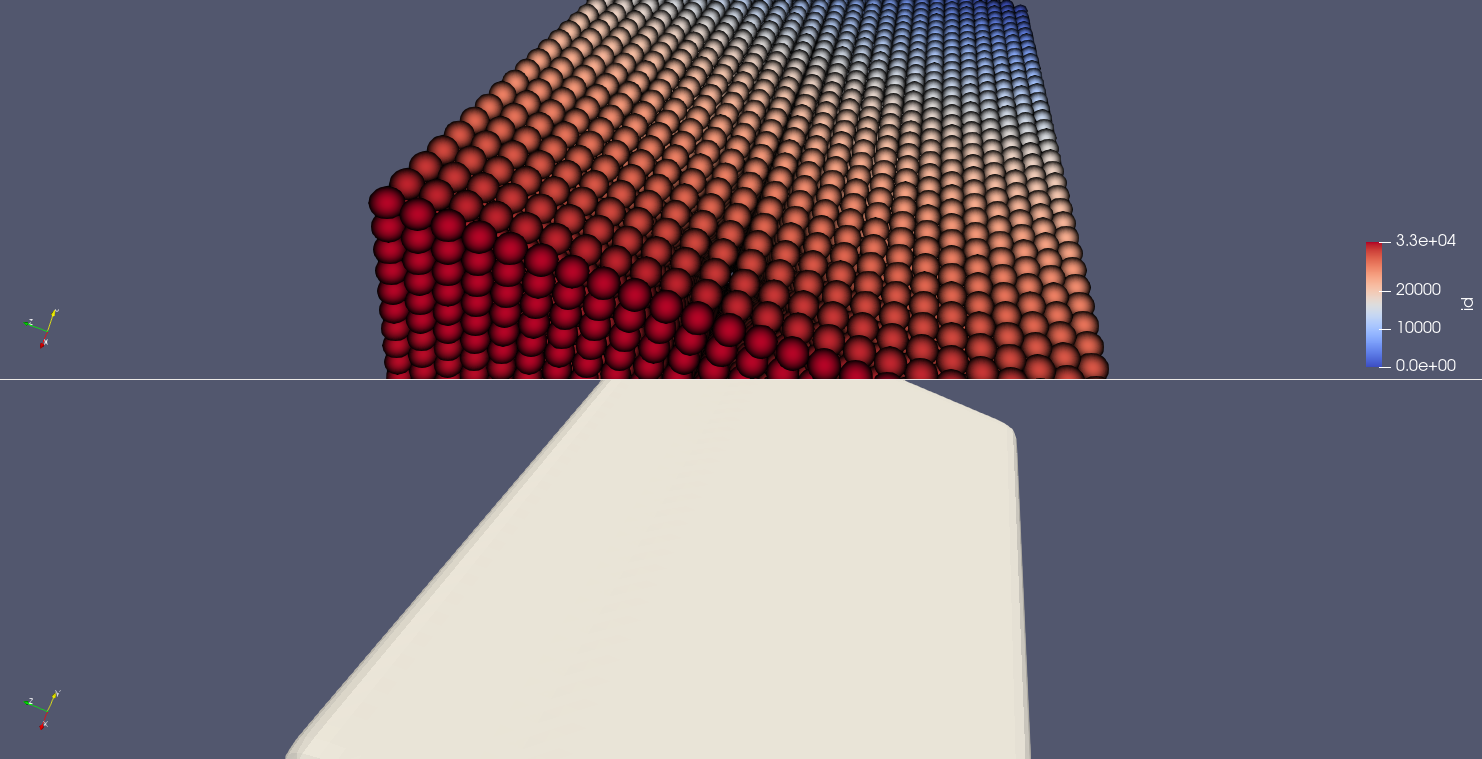
\includegraphics[width=\textwidth]{figures/FlatSurfaceWsParticleDisplacement.png}
			\caption{Regularly displaced particles}
		\end{subfigure}
		\begin{subfigure}[b]{0.6\textwidth}
			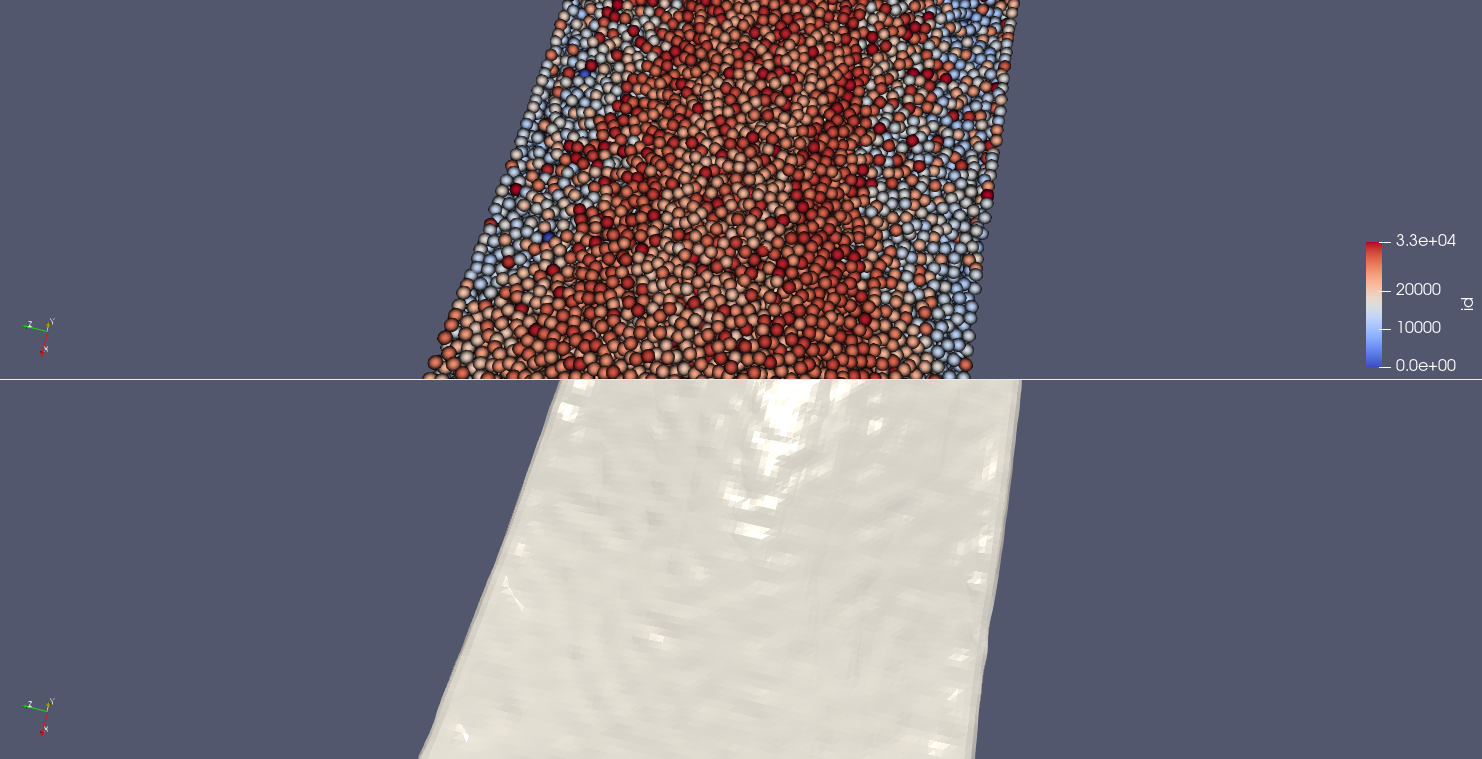
\includegraphics[width=\textwidth]{figures/NonFlatSurfaceWsParticleDisplacement.png}
			\caption{Irregularly displaced particles}
		\end{subfigure}
	\end{center}
	\caption{displacement of particles vs surface quality comparison}
	\label{fig:rec_vs_displacement}
\end{figure}
The main goal of this thesis is to develop a method, which will smooth out a high frequency bumps on flat surface areas, preserving the surface features. The first idea, that was applied to achieve this goal is simple blurring technique, which is extensively used in computer graphics, such as Gaussian Blur, Median blur, Bilateral blur or other image filtering techniques. In this chapter Blur-based method will be proposed to achieve the given goal. 
\section{Algorithm description}
Blur method was incorporated into the research framework according to the class hierarchy in Figure \ref{fig:class-diagam}. According to the class diagram, the method inherits the underlying base method (in our case its Density-Based, Zhu and Bridson, or Solenthaler methods), on top of which the computed level set is blurred.  Algorithm \ref{alg:blur_alg} shows the pseudo-code for \emph{updateLevelSet()}.
\begin{algorithm}[H]
	\scriptsize
	\begin{algorithmic}
		\State $levelSet \gets  BaseClass::initialLevelSet$
		\For{$i \in [0, blurIterations]$}
			\State blurLevelSet(levelSet);
		\EndFor
	\end{algorithmic}
	\caption{$updateLevelSet()$ for level set blurring method}
	\label{alg:blur_alg}
\end{algorithm}
According to Algorithm \ref{alg:blur_alg} blurring of the level set could be performed arbitrary number of times. The influence of number of iterations will be explained in further section.

The \emph{blurLevelSet()} pseudo-code is explained in Algorithm \ref{alg:blur_level_set}
\begin{algorithm}[H]
	\scriptsize
	\begin{algorithmic}
		\ForAll{$vtx \in MC\_CellDomain$}
			\State $neighbors \gets getNeighbourVertices(vtx);$
			\State $blurredLevelSetValue \gets 0$
			\ForAll{$nbVtx \in neighbors$}
				\State $blurredLevelSetValue\gets blurredLevelSetValue + levelSet[neighborVertex]$
			\EndFor
			\State $blurredLevelSetValue\gets\dfrac{blurredLevelSetValue}{sizeof(neighbors)}$
			\State $sf\gets computeSmoothingFactor()$
			\State $blurredLevelSet[vtx]\gets levecSet[vtx] * (1 - sf) + sf * blurredLevelSetValue;$
		\EndFor
	\end{algorithmic}
	\caption{$updateLevelSet()$ for level set blurring method}
	\label{alg:blur_level_set}
\end{algorithm}
The final blurred level set value in Algorythm \ref{alg:blur_level_set} is a wighted sum between the computed blur level set value and initial level set value.
\subsection{Smoothing factor}
The smoothing factor is a value that determines how much new, blurred level set value will contain initial level set value (weighted sum of blurred level set value and initial level set value). As described in \ref{alg:blur_level_set} level set value is updated according to the Equation \ref{eq:level_set_value}.
\begin{equation}
newLS = oldLS \cdot (1 - sf) + blurLS \cdot sf \label{eq:level_set_value}
\end{equation}
In Equation \ref{eq:level_set_value} $sf$ is a smoothing factor or a weight. The smoothing factor itself is calculated according to equation \ref{eq:smooth_factor}.
\begin{equation}
	sf_{vtx} = 1 - (1 - min(1, \dfrac{bsf \cdot fp_{vtx}}{maxFp})^2)^{10} \label{eq:smooth_factor}
\end{equation}
where:
\begin{conditions}
	vtx & vertex for which the smoothing factor is computed\\
	fp_{vtx} & number of neighbor fluid particles within support radius from vtx\\
	maxFp & maximum possible fluid particles that can be in the neighborhood of the vertex \\
	bsf & base support factor (use defined)
\end{conditions}
The smoothing factor formula was designed such that it should be maximal for vertices that contains full fluid particles set and minimum where number of fluid particles limits to zero (see Figure \ref{fig:sf_function_graph}).
\begin{figure}[H]
	\begin{center}
			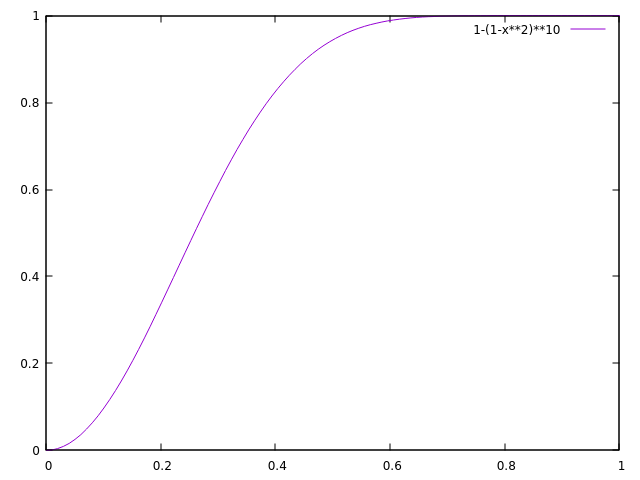
\includegraphics[width=0.5\textwidth]{figures/sf_function_graph.png}		
	\end{center}
	\caption{Graphic of function, representing equation \ref{eq:smooth_factor}. Taking into account that $min(1, \dfrac{bsf \cdot fp_{vtx}}{maxFp}) \in [0,1]$ the function converges from 0 to 1 in the interval $x \in [0, 0.5]$ and limits to 1 for the area $x\in [0.5, 1]$}
	\label{fig:sf_function_graph}
\end{figure}


The motivation to apply such a smoothing factor comes from the problem of the blurring algorithm. If we apply the blur algorithm uniformly into all MC vertex domains, the blur will smooth out the features in thin areas and the areas with a small set of particles (droplets or splashes). Figure \ref{fig:smoothing_factor_influence} shows the problem of application of the blur algorithm w.o. application of smoothing factor.

\begin{figure}[H]
	\begin{center}
			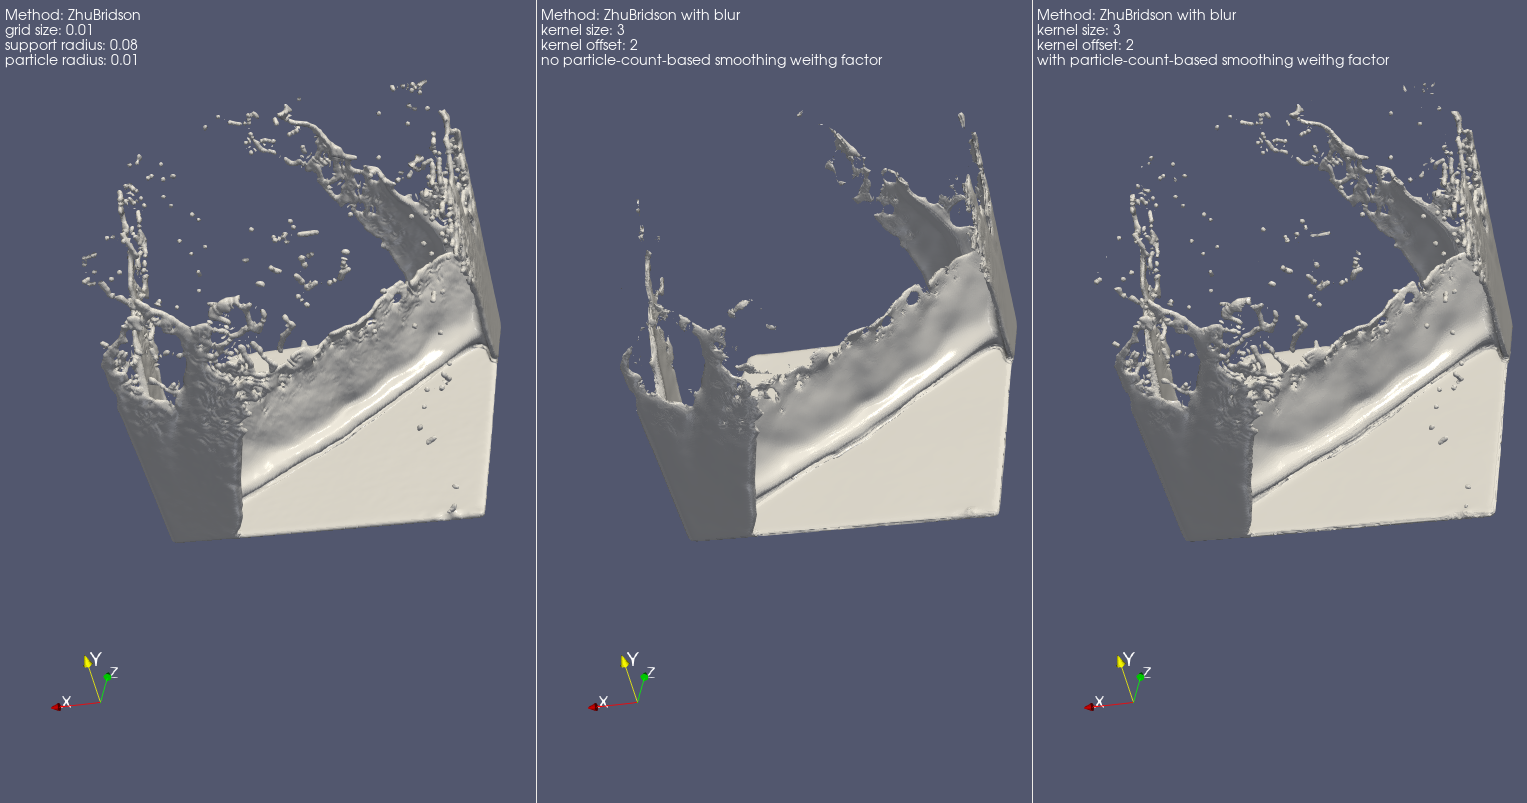
\includegraphics[width=\textwidth]{figures/View2.png}		
	\end{center}
	\caption{Leftmost is initial Zhu and Bridson reconstruction, middle - blur reconstruction w.o. smoothing factor application, rightmost - blur reconstruction with usage of smoothing factor}
	\label{fig:smoothing_factor_influence}
\end{figure}


The idea of blurring using a smoothing factor is to blur the level set as much as possible in the areas where the surface of the fluid is flat and to apply less blur in areas, where a set of MC cells lacks fluid particles. Suppose the general case in Figure \ref{fig:sf_example}. In the figure red and yellow grid, vertices contain a full and half set of particles respectively. Level set values of the grid points are supposed to be blurred as much as possible.
\begin{figure}[H]
	\begin{center}
		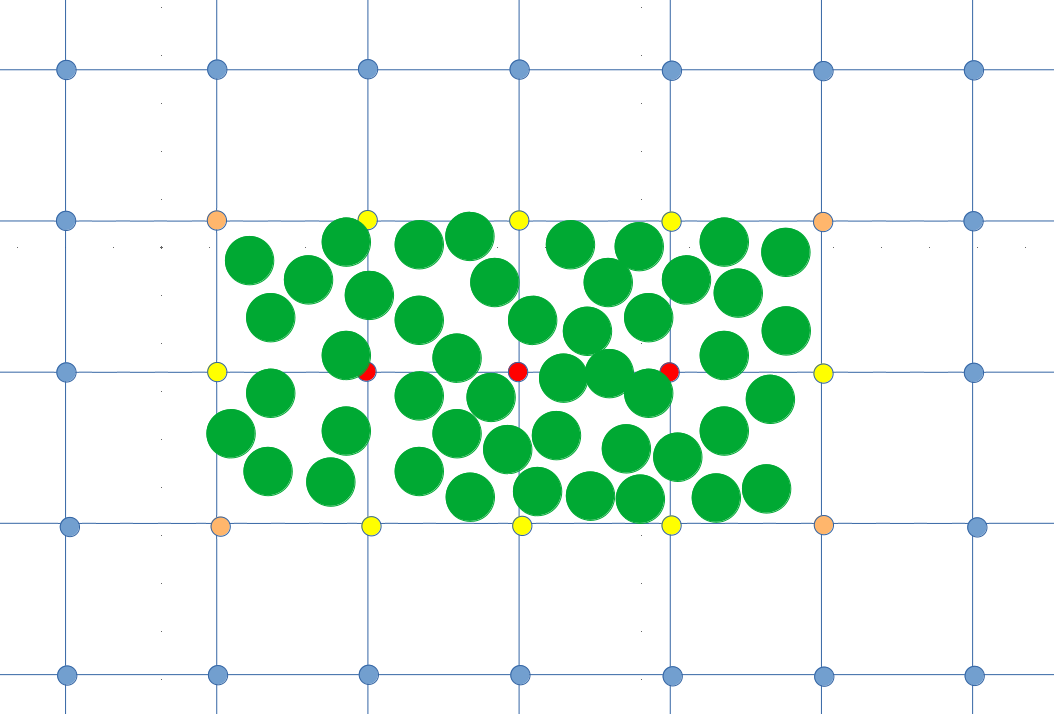
\includegraphics[width=0.5\textwidth]{figures/SmoothingFactorPictureExplenation.png}		
		\caption{Green circles are fluid particles, red - MC cells with full set of fluid particles in the neighborhood, yellow -  MC cells with half set of fluid particles in the neighborhood, orange - MC cells with quarter set of fluid particles in the neighborhood, blue - MC cells with no fluid particles in the neighborhood}
		\label{fig:sf_example}
	\end{center}
\end{figure}
Applying blur to the level set vertices that are inside the fluid (and all its neighbor cells are also inside the fluid) will not change the level set value too much as soon all vertices that has full set of fluid particles in the neighborhood will have similar level set values. 
For the MC vertices that are near the corners the 75\% of the neighbor vertices are outside the fluid, which will bias the vertex outside the fluid, thus the fluid will shrink. This is also relevant for the thin areas and splashes.\\
At the figure \ref{fig:blur_w_o_sf} the effect of surface shrinkage of applying blur in the thin area and in the corners w.r.t. the initial reconstruction method can be observed. The flat surface is smoothed out, but at the same time surface at the thin and splash areas is degraded, some small features/droplets are lost.
\begin{figure}[H]
	\begin{center}
		\begin{subfigure}[b]{\textwidth}
			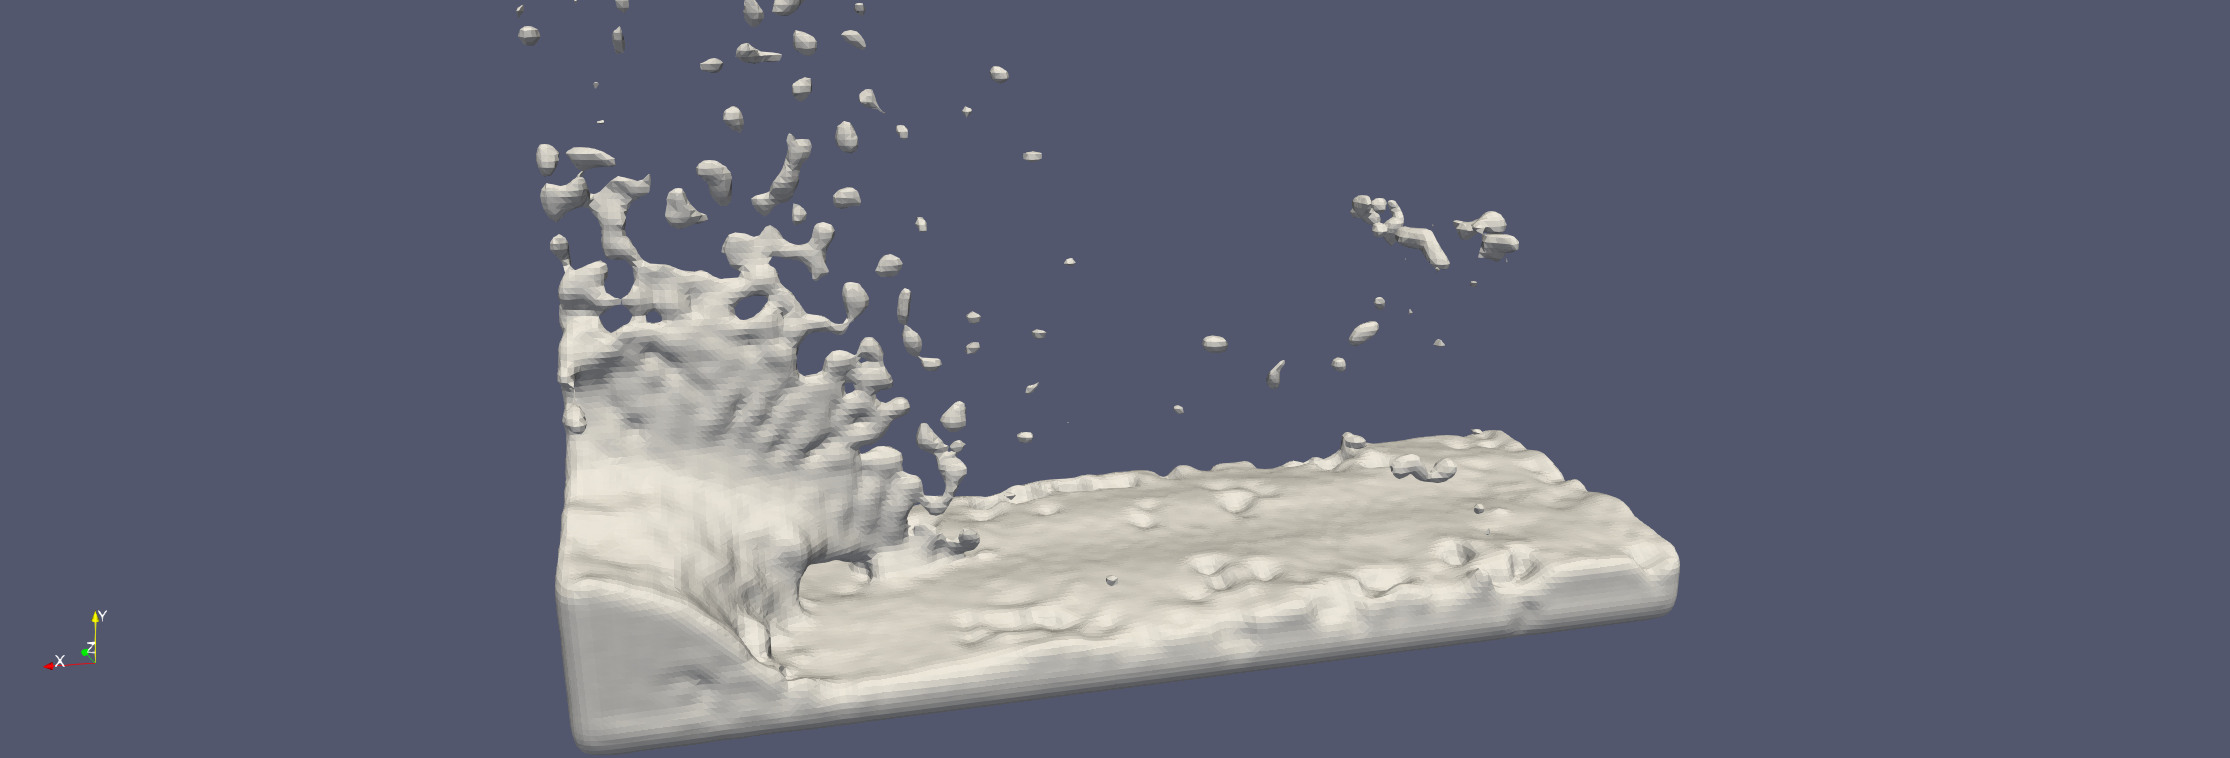
\includegraphics[width=\textwidth]{figures/DenvityBlurredSplashArea.png}
			\caption{Density based surface reconstruction}
			\label{fig:denc_rec}
		\end{subfigure}
		\begin{subfigure}[b]{\textwidth}
			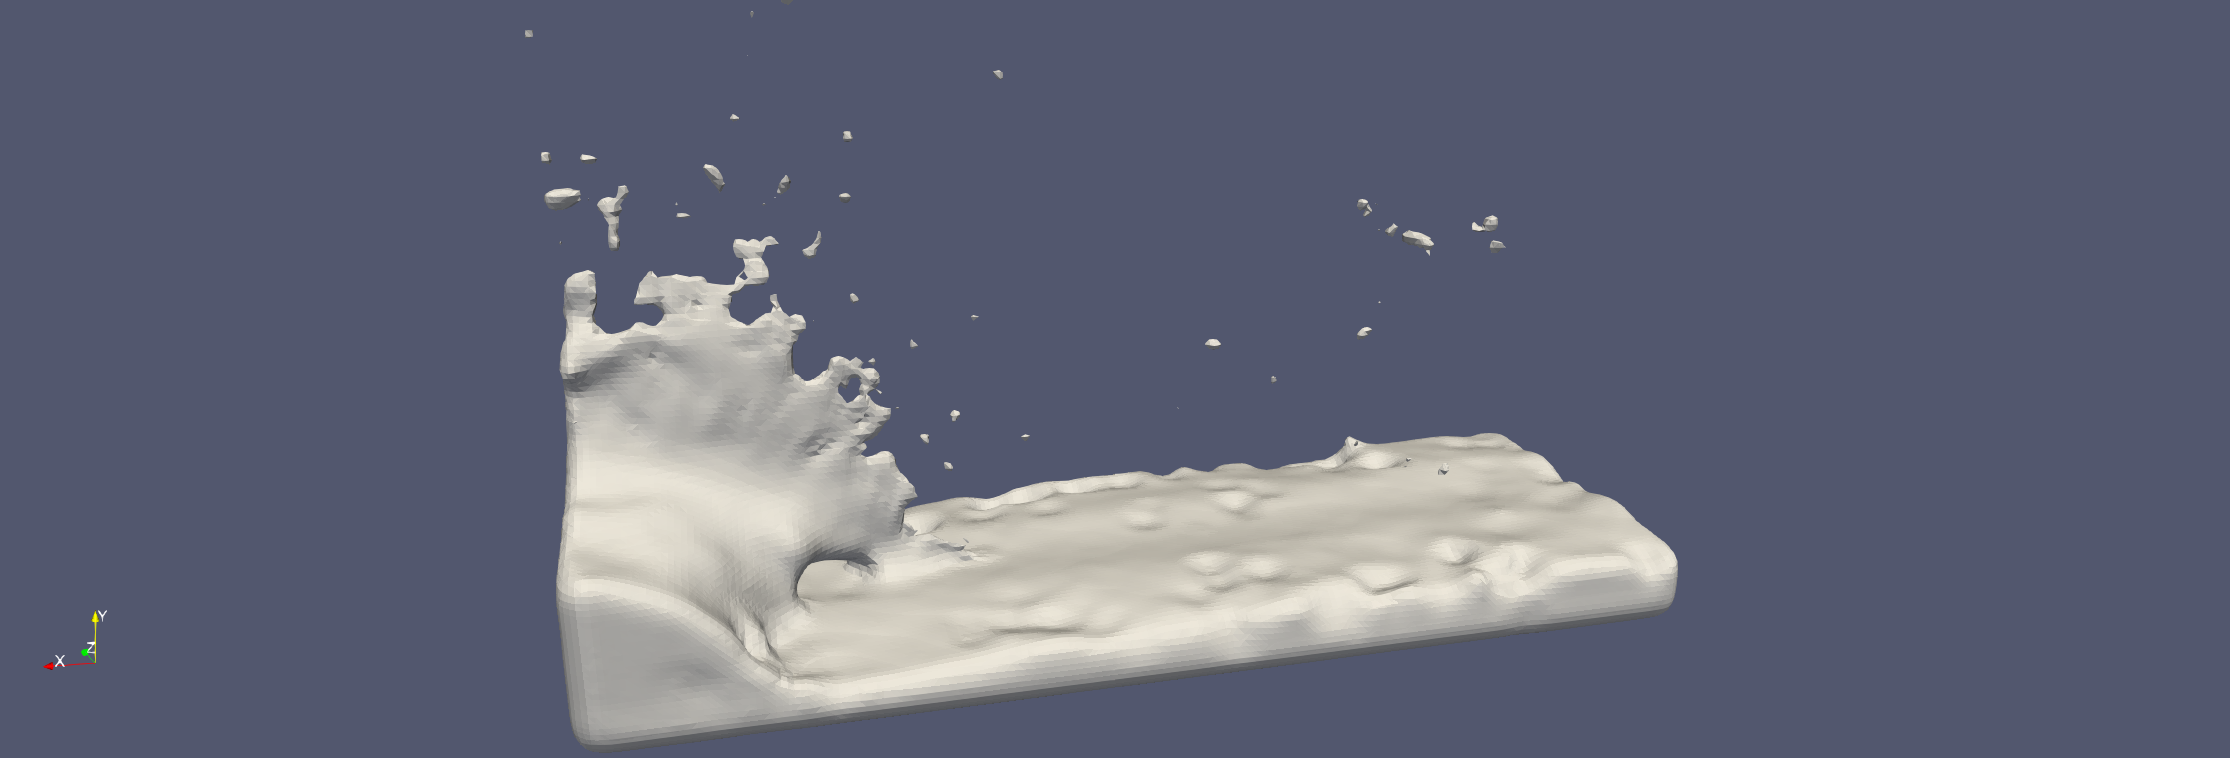
\includegraphics[width=\textwidth]{figures/DenvityBasedSplashArea.png}
			\caption{Density based surface reconstruction with blur (smoothing factor is not applied)}
			\label{fig:blur_w_o_sf}
		\end{subfigure}
	\end{center}
	\caption{Comparison of original reconstruction method and blurred reconstruction without application of smoothing factor}
	\label{fig:blur_thin_area}
\end{figure}
In the other hand applying blur on level set with smoothing factor smooths out the flat surface areas bumps, but preserves small feature areas (see Figure \ref{fig:blur_thin_area_with_sf}).
\begin{figure}[H]
        \begin{subfigure}[b]{0.5\textwidth}
               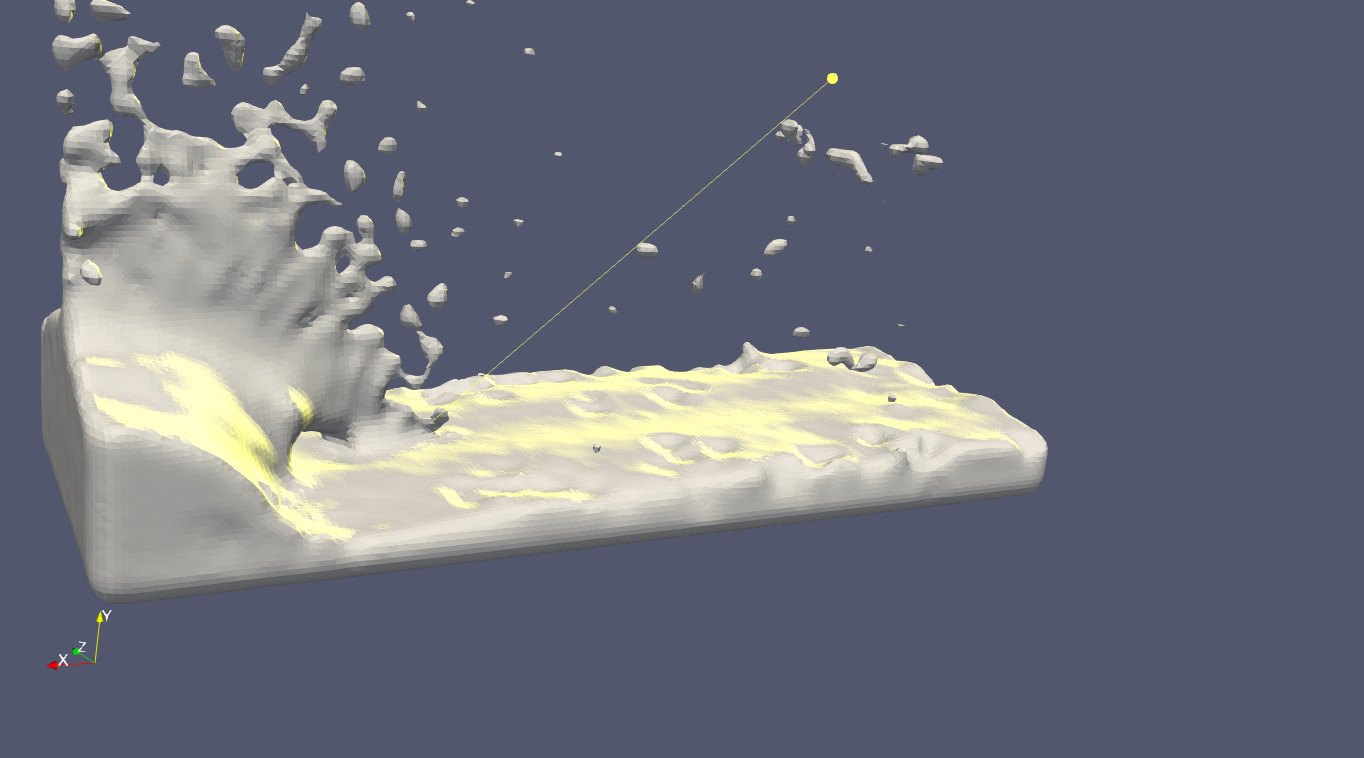
\includegraphics[width=\textwidth]{figures/DenvityBasedSplashArea2.png}
               \caption{Density based surface}
               \label{fig:db_rec}
        \end{subfigure}
        \begin{subfigure}[b]{0.5\textwidth}
               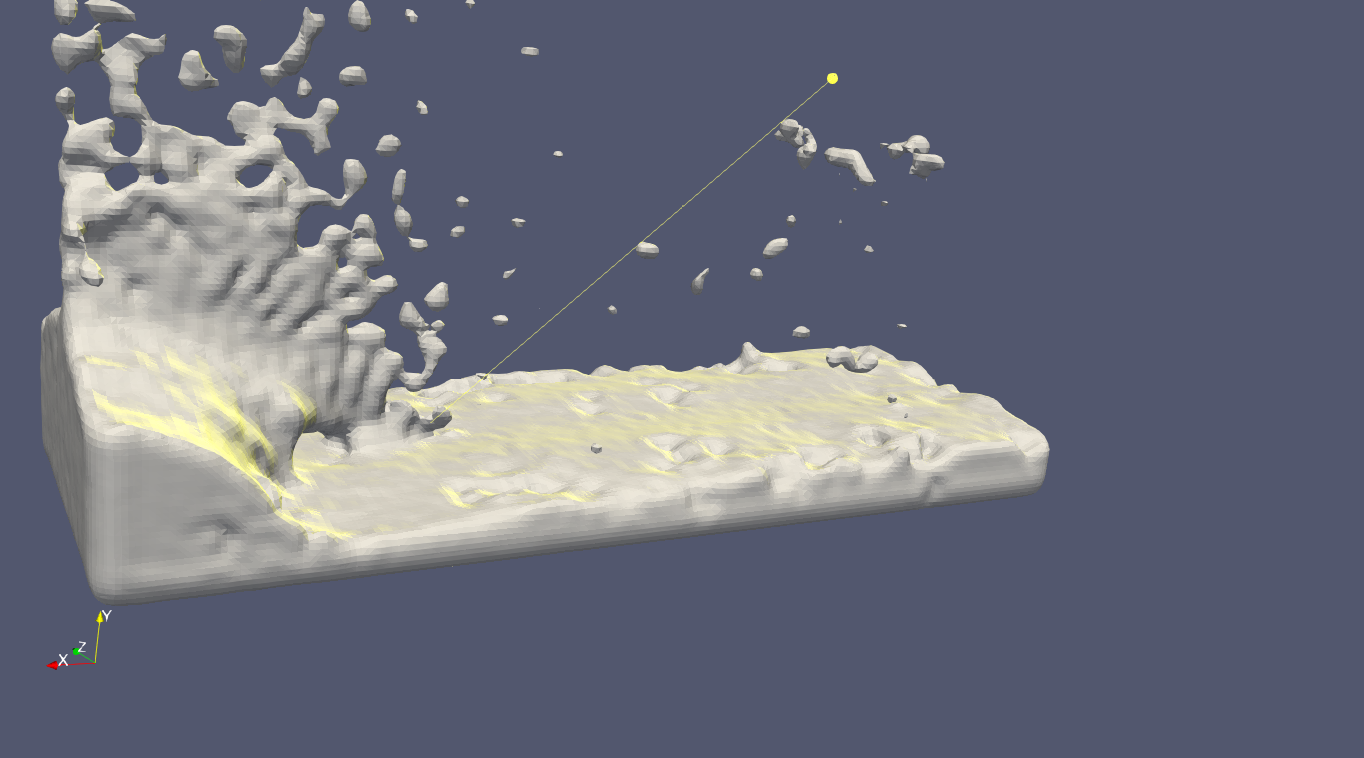
\includegraphics[width=\textwidth]{figures/DenvityBlurredSplashArea2.png}
               \caption{Applying smoothing factor to level set blur}
				\label{fig:blur_with_sf}
        \end{subfigure}
       \caption{Comparison of original reconstruction method and blurred reconstruction with application of smoothing factor}
       \label{fig:blur_thin_area_with_sf}
 \end{figure}
 \subsection{Neighbors detection algorithm}
In the Algorithm \ref{alg:blur_level_set} MC neighbor vertices are computed in function $getNeighbourVertices(vtx)$. The Algorithm \ref{alg:blur_nbs_search} describes the procedure of neighbors detection procedure.
\begin{algorithm}[H]
	\scriptsize
	\begin{algorithmic}
		\State $neighbors \gets \{vtx\}$
		\State $sdfGradient \gets \nabla_x sdf(vtx)$
		\If{$sdfGradient \cdot sdfGradient < 1e-6$}
			\State $return\ neighbors$
		\EndIf
		\State $Normalize sdfGradient$
		
		\For{$i \in [-kernelSize \cdot kernelOffset, kernelSize \cdot kernelOffset]$, $stepsize = kernelOffset$}
			\For{$j \in [-kernelSize \cdot kernelOffset, kernelSize \cdot kernelOffset]$, $stepsize = kernelOffset$}
				\For{$k \in [-kernelSize \cdot kernelOffset, kernelSize \cdot kernelOffset]$, $stepsize = kernelOffset$}
					\If{$i = 0 \land j = 0 \land k = 0$}
						\State $neighbors \gets neighbors \cup vtx$
						\State $continue$
					\EndIf
					
					\State $offsetVector \gets [i \cdot GridResolution, j \cdot GridResolution, k \cdot GridResolution]$;
					\If{$offsetVector \cdot sdfGradient \geq kernelDepth \cdot kernelSize \cdot GridResolution$}
						\State $continue$
					\EndIf
					
					\State $neighbors \gets neighbors \cup (vtk + offsetVector)$
				\EndFor
			\EndFor
		\EndFor
		\State $return\ neighbors$
	\end{algorithmic}
	\caption{neighborhood search for level set blur algorithm}
	\label{alg:blur_nbs_search}
\end{algorithm}
\subsection{Blur kernel size and offset}
\textcolor{red}{TODO}

\subsection{Kernel depth}
The advantage of the static MC grid is that it has a static displacement of all grid vertices, thus the neighborhood can be efficiently computed. However, using the full neighborhood within the $kernelSize$ and $kernelOffset$ is not sufficient for level set blurring. As soon as the smoothing aims to remove bumps in the flat surface areas it is more practical to take into account level set vertices, that are in the neighborhood of the fluid surface. Thus, for each vertex of the level set gradient of the level set can be computed, and the gradient vector is normal to the fluid surface \cite{LevelSetMethods}. Thus for the flat surface areas, it is convenient to blur level set vertex value w.r.t. vertices, which resides in a tangential direction to the surface normal.

\begin{figure}[H]
        \begin{subfigure}[b]{0.5\textwidth}
               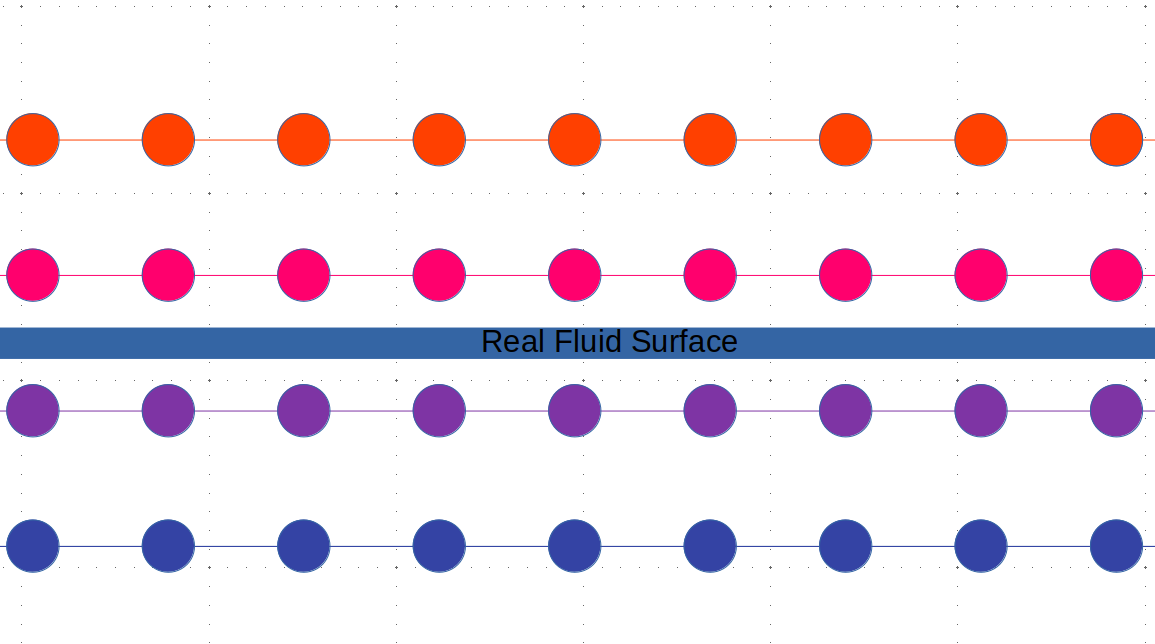
\includegraphics[width=\textwidth]{figures/RealFluidSurfaceLevelSet.png}
               \caption{Expected reconstruction of flat surface}
               \label{fig:expected_fs}
        \end{subfigure}
        \begin{subfigure}[b]{0.5\textwidth}
               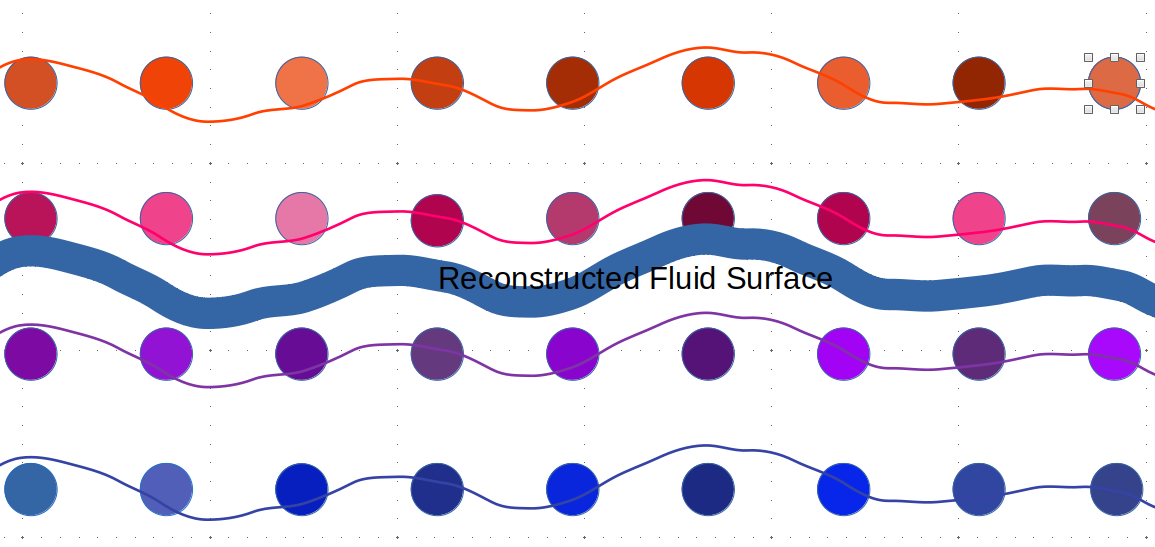
\includegraphics[width=\textwidth]{figures/ReconstructedFluidSurface.png}
               \caption{Bumpy reconstruction of flat surface}
				\label{fig:recon_fs}
        \end{subfigure}
        \begin{subfigure}[b]{0.5\textwidth}
               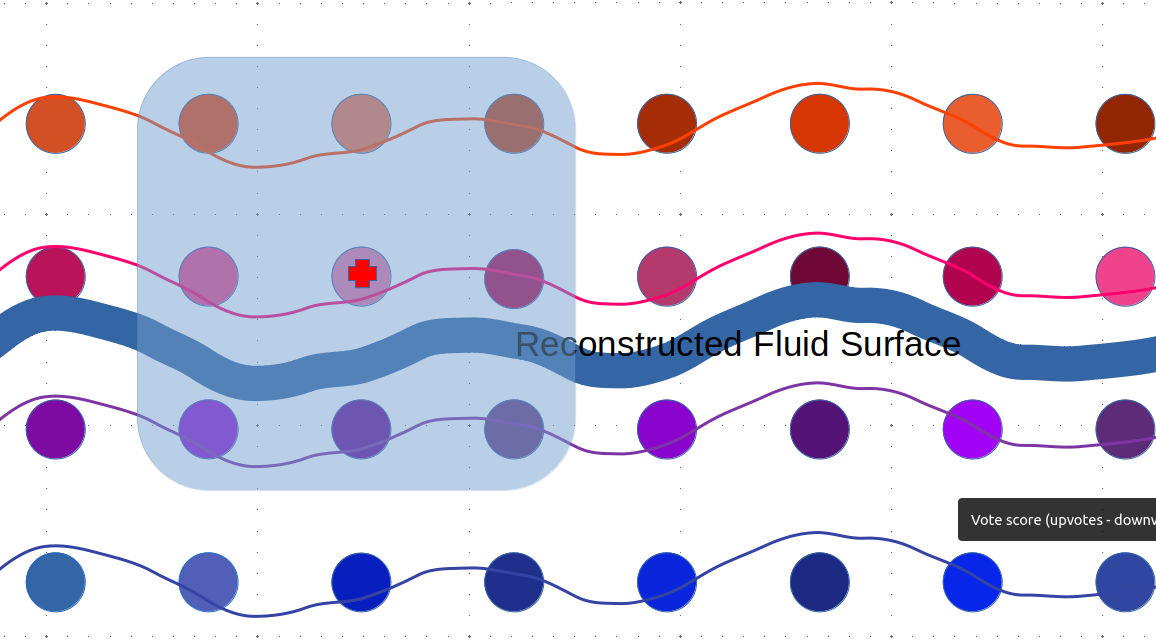
\includegraphics[width=\textwidth]{figures/LevelSetBlurFullKernel.png}
               \caption{Application of full kernel size}
               \label{fig:full_ks}
        \end{subfigure}
        \begin{subfigure}[b]{0.5\textwidth}
               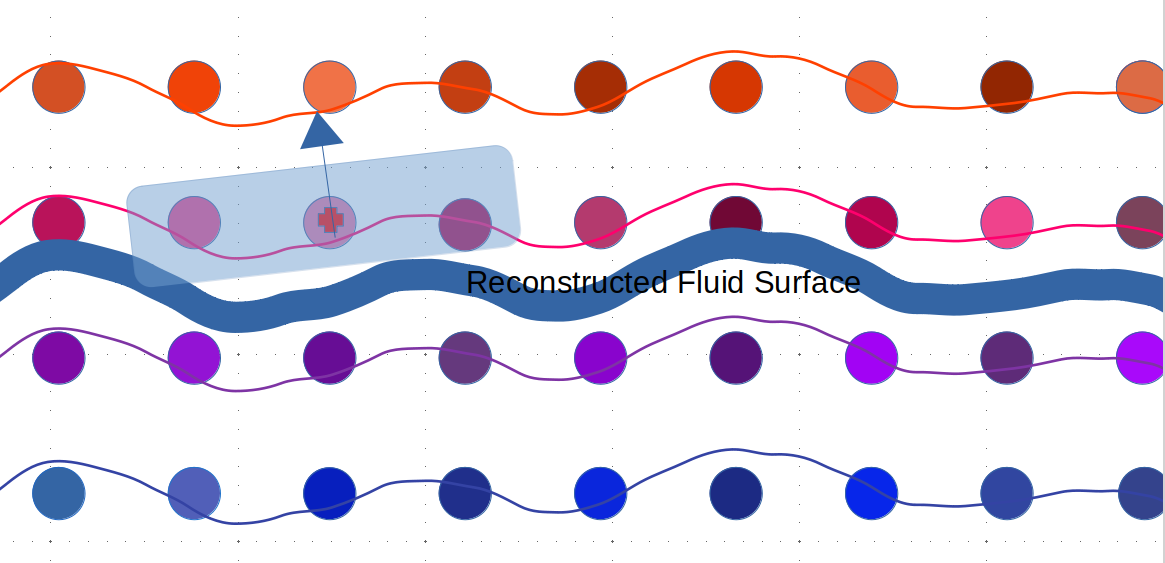
\includegraphics[width=\textwidth]{figures/LevelSetBlurKernelPart.png}
               \caption{Adjustment kernel in normal direction to iso-surface}
				\label{fig:partial_ks}
        \end{subfigure}

       \caption{Colored lines are iso-surface levels. Dots are MC grid vertices with their respective level set values}
       \label{fig:kd_surface_explenation}
 \end{figure}
At the Figure \ref{fig:expected_fs} expected iso-surface in flat fluid area is displayed. Dots of different colors are the MC grid vertices. Colors represent the level set value. In the perfect case level set ISO-lines (in the 2D example) forms straight lines, thus MC grid vertices along the iso-line will receive similar values. However, due to the irregular displacement of fluid particles surface is usually reconstructed as shown in Figure \ref{fig:recon_fs}. In case if we apply full kernel size (see Figure \ref{fig:full_ks}) we will pick level set values from different iso-surface levels, which will change level set values unpredictably.\\
The better approach is to pick a kernel frame so that only level set values of near-surface MC vertices will be used for blur operation (Figure \ref{fig:partial_ks}). This way blur operation will smooth out grid vertices along the iso lines. Especially the influence of the kernel depth can be seen in thin areas, where kernel frame is larger than a thickness of a fluid surface (see Figure \ref{fig:kd_influence example}).
\begin{figure}[H]
        \begin{subfigure}[b]{1\textwidth}
               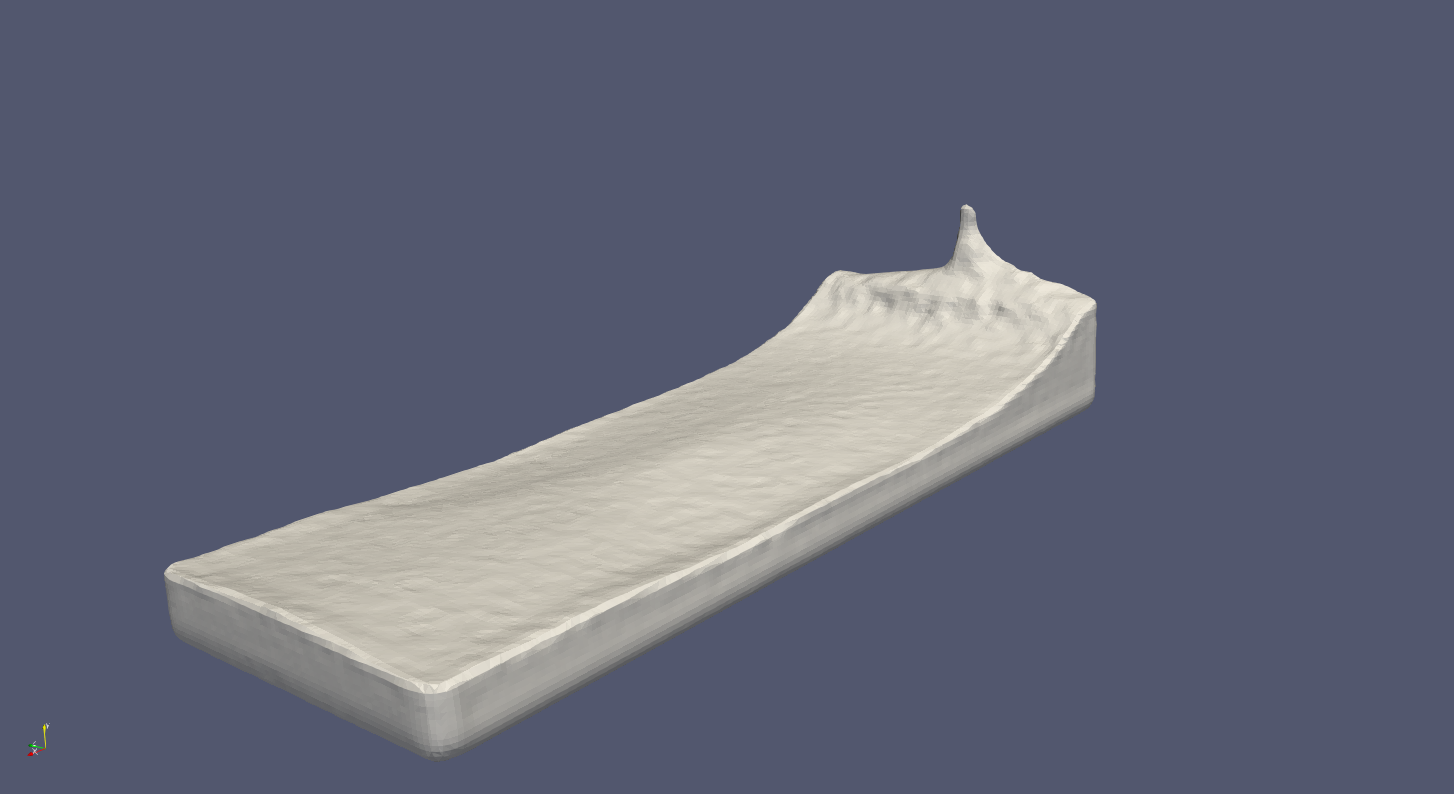
\includegraphics[width=\textwidth]{figures/KernelDepthOriginalReconstruction.png}
               \caption{Original ZhuBridson reconstruction}
               \label{fig:kd_original}
        \end{subfigure}
        \begin{subfigure}[b]{0.5\textwidth}
               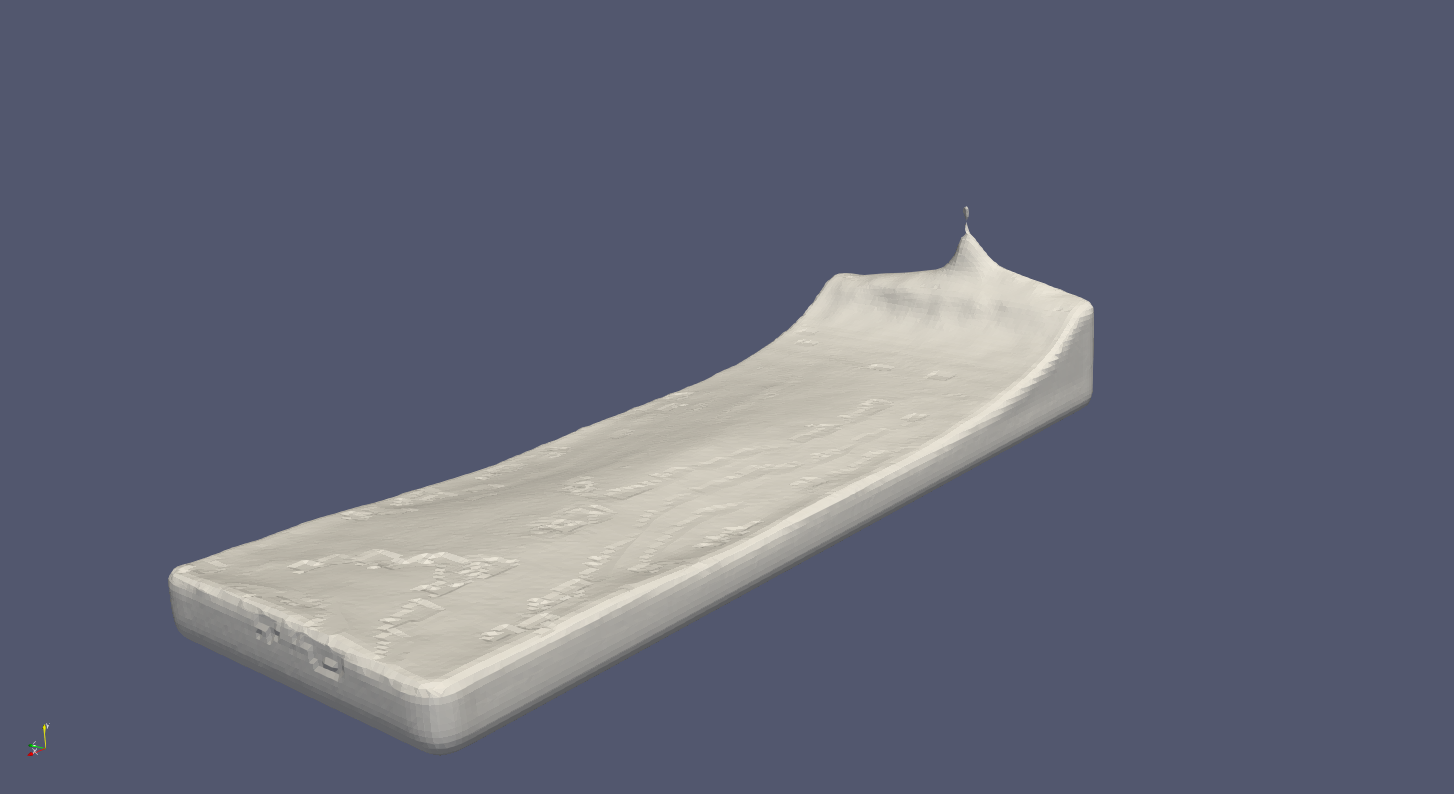
\includegraphics[width=\textwidth]{figures/KernelDepth1.png}
               \caption{Blur with full kernel size}
				\label{fig:kd_full}
        \end{subfigure}
        \begin{subfigure}[b]{0.5\textwidth}
               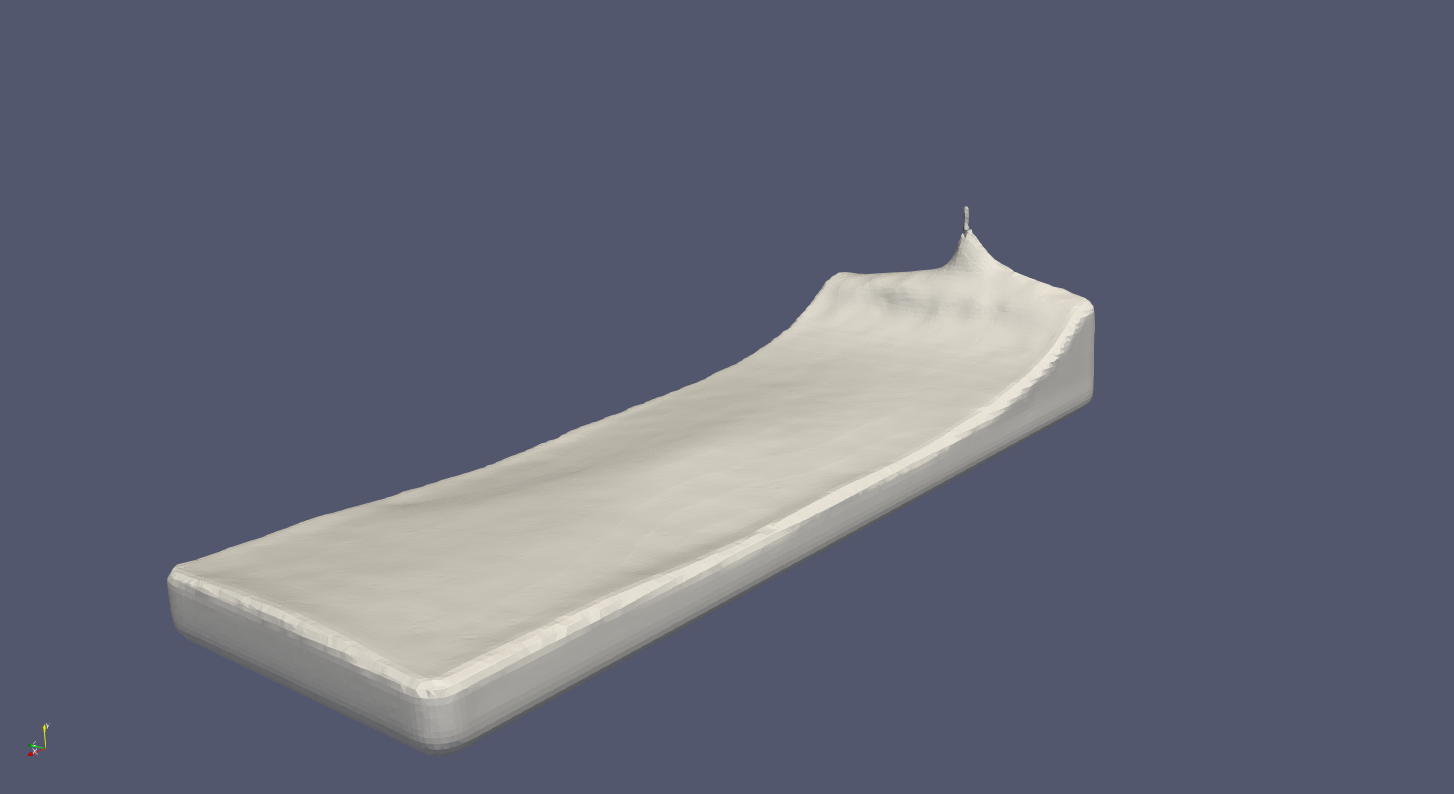
\includegraphics[width=\textwidth]{figures/KernelDepth0_5.png}
               \caption{Blur with half kernel size}
               \label{fig:kd_half}
        \end{subfigure}

       \caption{Influence of the kernel depth on level set blurring}
       \label{fig:kd_influence example}
 \end{figure}


\section{Blur Iterations}
Apart to other parameters it was decided to check the influence of application of blur iteratively to the level set. In the Algorithm \ref{alg:blur_alg} blur applied iteratively on the level set. The results of the iterative blur can be observed on the Figure \ref{fig:bi_reconstruction}. The higher number of blur iterations the smother resulting surface becomes. 
\begin{figure}[H]
        \begin{subfigure}[b]{0.5\textwidth}
               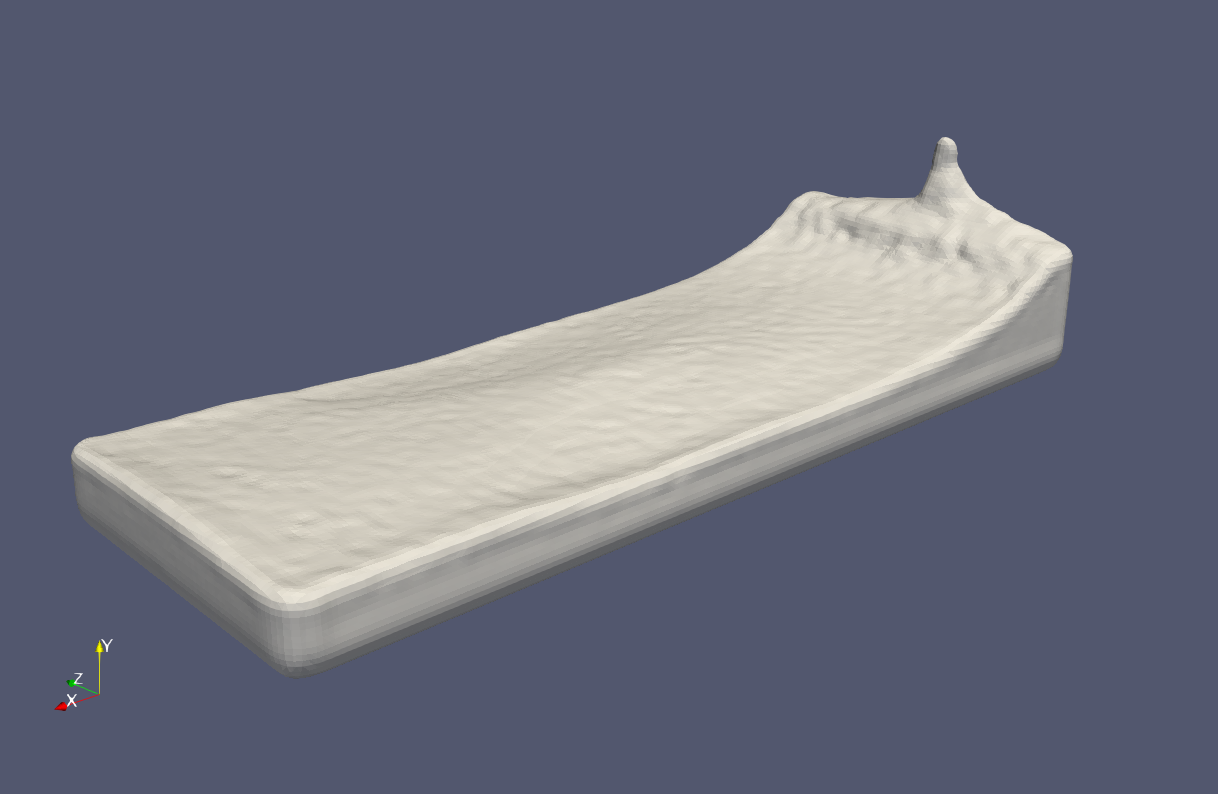
\includegraphics[width=\textwidth]{figures/ReconstructionIterations0.png}
				\caption{0 blur iterations}
               \label{fig:bi_original}
        \end{subfigure}
        \begin{subfigure}[b]{0.5\textwidth}
               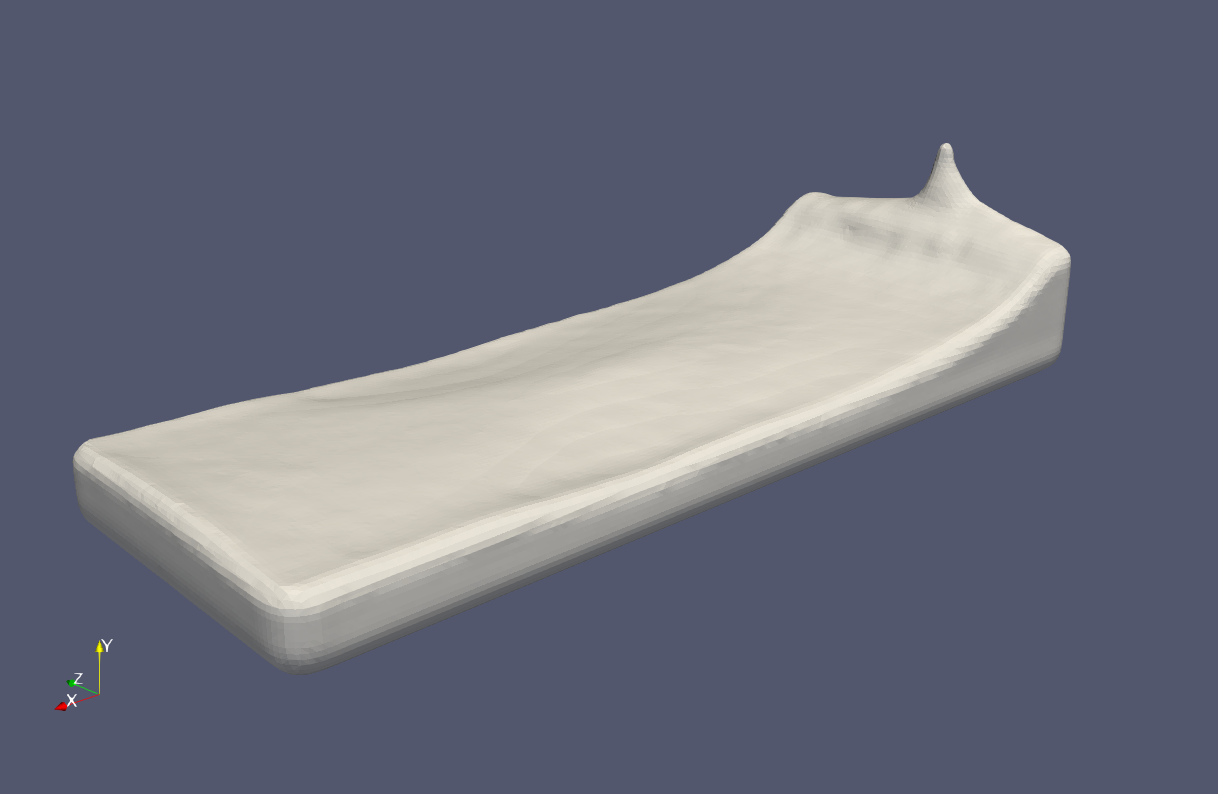
\includegraphics[width=\textwidth]{figures/ReconstructionIterations1.png}
				\caption{1 blur iterations}

				\label{fig:bi_1iteration}
        \end{subfigure}
        \begin{subfigure}[b]{0.5\textwidth}
               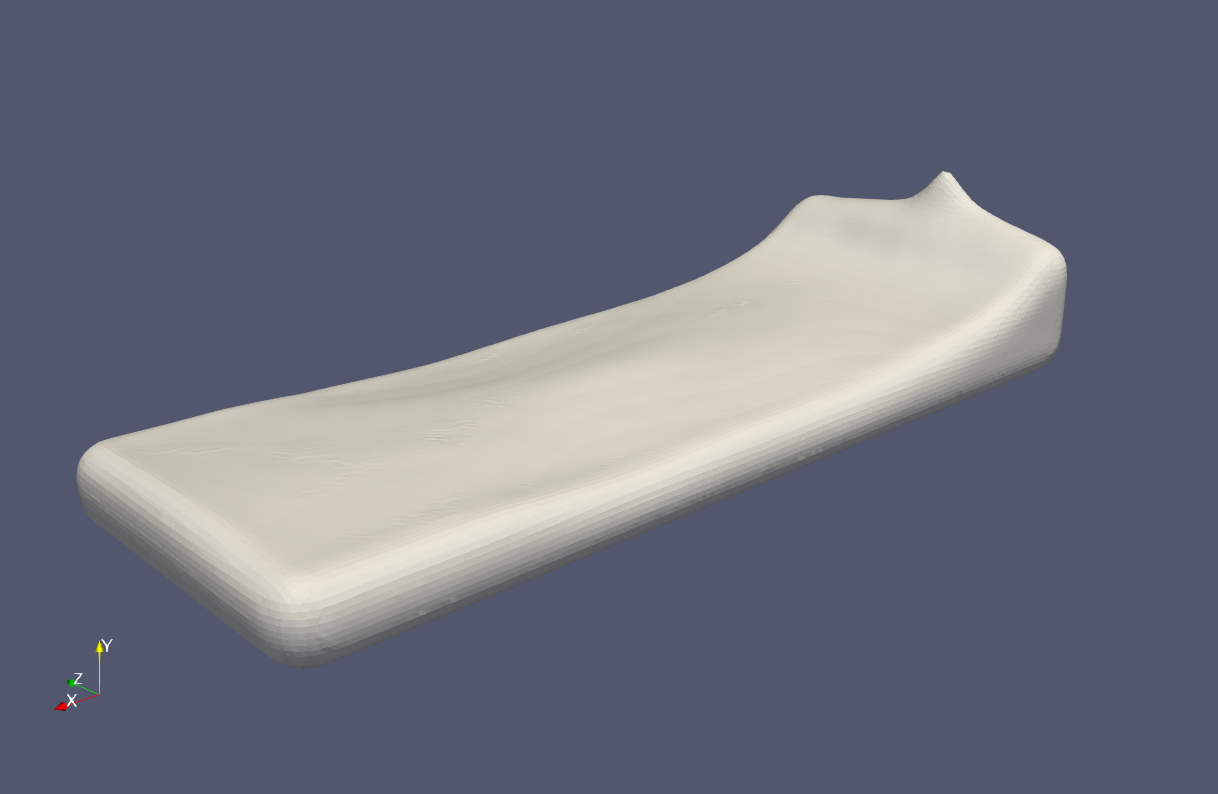
\includegraphics[width=\textwidth]{figures/ReconstructionIterations4.png}
				\caption{4 blur iterations}
               \label{fig:bi_4iteration}
        \end{subfigure}
        \begin{subfigure}[b]{0.5\textwidth}
               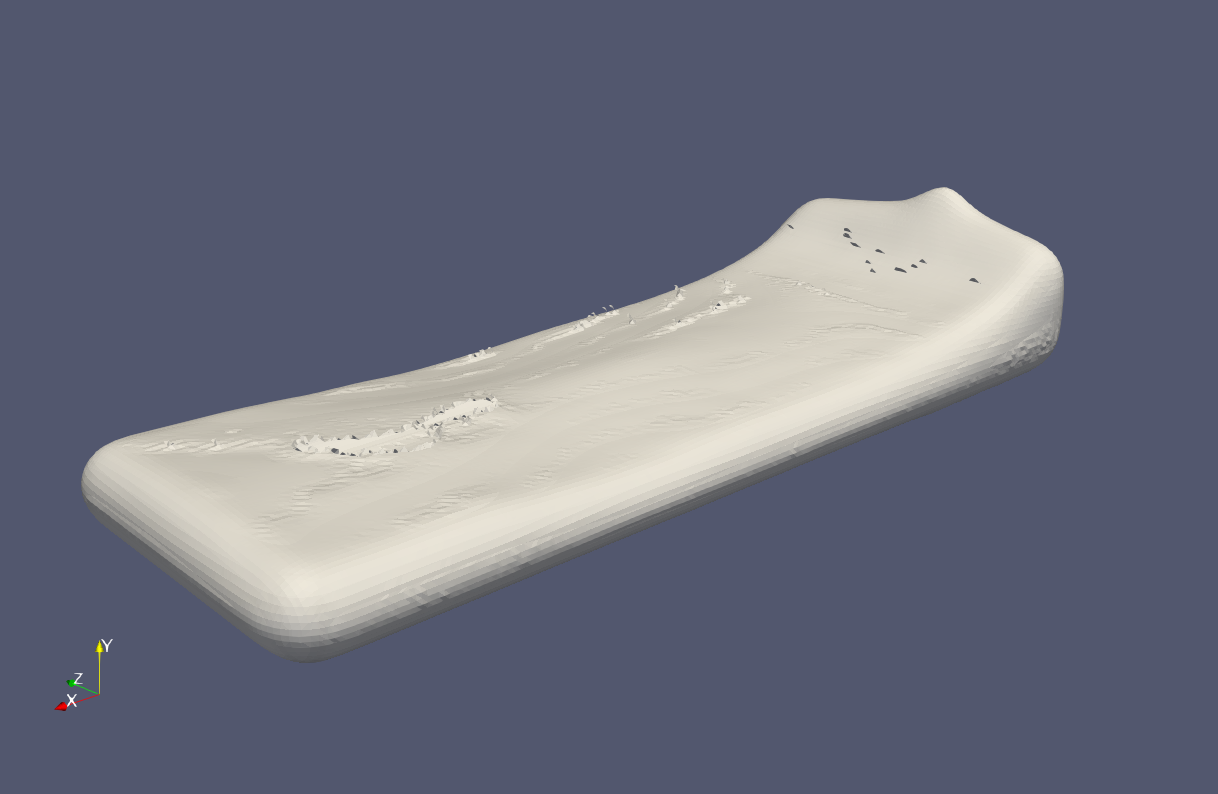
\includegraphics[width=\textwidth]{figures/ReconstructionIterations8.png}
				\caption{8 blur iterations}
               \label{fig:bi_8iteration}
        \end{subfigure}
       \caption{Reconstructed surface depending on the number of blur iterations}
       \label{fig:bi_reconstruction}
\end{figure}
However, large amount of iterations smooths out level set to uniform value, thus on the Figure \ref{fig:bi_8iteration} holes can be seen. Figure \ref{fig:bi_levelset} displays the influence of blur iterations on level set itself. 
\begin{figure}[H]
        \begin{subfigure}[b]{0.5\textwidth}
               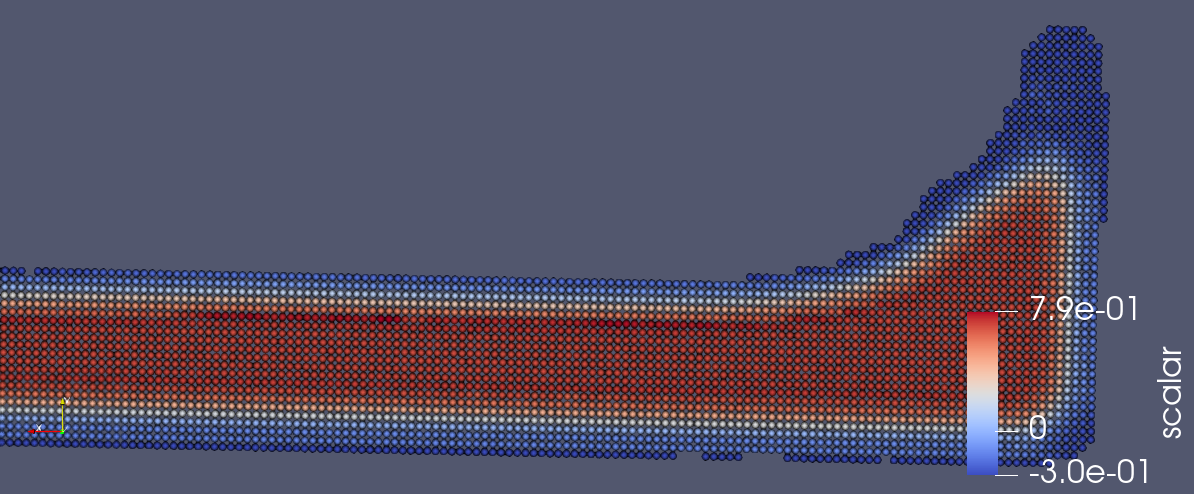
\includegraphics[width=\textwidth]{figures/LevelSetBlurIterations4.png}
				\caption{4 blur iterations}
               \label{fig:ls_bi_original}
        \end{subfigure}
        \begin{subfigure}[b]{0.5\textwidth}
               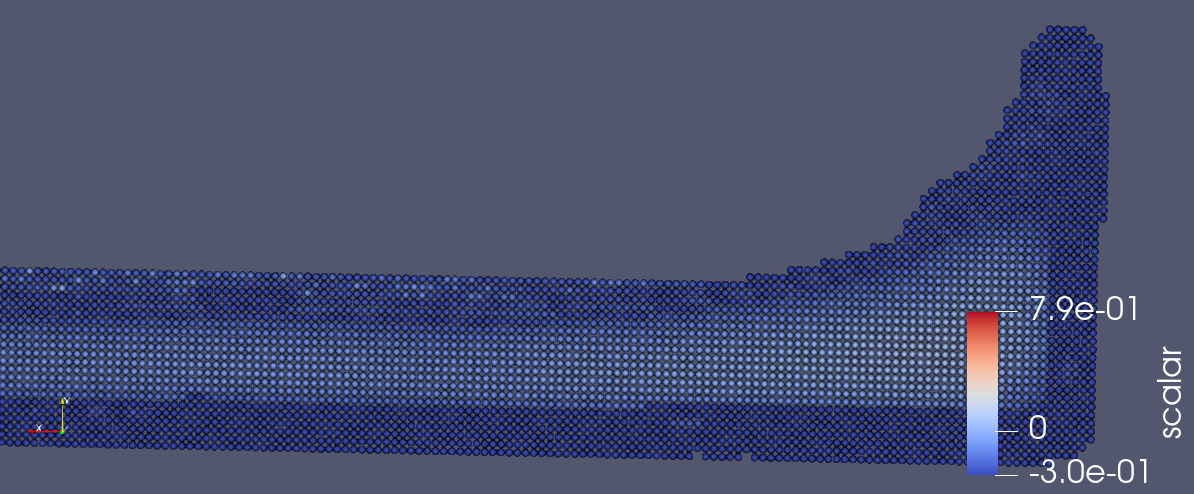
\includegraphics[width=\textwidth]{figures/LevelSetBlurIterations16.png}
				\caption{16 blur iterations}

				\label{fig:ls_bi_16iteration}
        \end{subfigure}
       \caption{Level set depending on the number of blur iterations}
       \label{fig:bi_levelset}
\end{figure}

An important property of the blur reconstruction algorithm should be noted. Lets analyze the blur algorithm, applied on the level set (for simplicity 2D version will be analyzed).\\
Suppose matrix $A = 
\begin{pmatrix}
	1 & 1 & ... & 1\\
	1 & 1 & ... & 1\\
	. & . & ... & .\\
	1 & 1 & ... & 1\\
\end{pmatrix}$ is a $n \times n$ kernel where n is odd.
Kernel multiplication operation on level set element is described in equation \ref{eq:kernel-operation}
\begin{equation}
	\dfrac{1}{n^2}\cdot A\cdot sdf_{ij} = \sum_{k=- \left \lfloor{n/2}\right \rfloor}^{\left \lfloor{n/2}\right \rfloor}
		{\sum_{l=- \left \lfloor{n/2}\right \rfloor}^{\left \lfloor{n/2}\right \rfloor}{ A_{k+1, l+1} \cdot sdf_{i+k, j+l}}}
	\label{eq:kernel-operation}
\end{equation}
Suppose $n=3$ and $ sdf^{(k)}_{i,j} = \dfrac{1}{9} \cdot A \cdot sdf^{(k-1)}_{i,j} = \dfrac{1}{9^k} \cdot A^{(k)} \cdot sdf^{(0)}_{i,j}$\\. The claim is that $A^{(k)}$ satisfies properties of a kernel function (\ref{SPHtechniques}):
\begin{itemize}
	\item normalization condition
	\item positivity condition
	\item symmetry condition
	\item compact support condition
\end{itemize}
\textcolor{red}{TODO: PROOF}\\
E.g. $A^2 = 
\begin{pmatrix}
1 & 2 & 3 & 2 & 1\\
2 & 4 & 6 & 4 & 2\\
3 & 6 & 9 & 6 & 3\\
2 & 4 & 6 & 4 & 2\\
1 & 2 & 3 & 2 & 1\\
\end{pmatrix}$
$A^3 = 
\begin{pmatrix}
 1 & 3 & 6 & 7 & 6 & 3 & 1\\
 3 & 9 & 18 & 21 & 18 & 9 & 3\\
 6 & 18 & 36 & 42 & 36 & 18 & 6\\
 7 & 21 & 42 & 49 & 42 & 21 & 7\\
 6 & 18 & 36 & 42 & 36 & 18 & 6\\
 3 & 9 & 18 & 21 & 18 & 9 & 3\\
 1 & 3 & 6 & 7 & 6 & 3 & 1\\
\end{pmatrix}$\\
$A^4 = 
\begin{pmatrix}
1 & 4 & 10 & 16 & 19 & 16 & 10 & 4 & 1\\
4 & 16 & 40 & 64 & 76 & 64 & 40 & 16 & 4\\
10 & 40 & 100 & 160 & 190 & 160 & 100 & 40 & 10\\
16 & 64 & 160 & 256 & 304 & 256 & 160 & 64 & 16\\
19 & 76 & 190 & 304 & 361 & 304 & 190 & 76 & 19\\
16 & 64 & 160 & 256 & 304 & 256 & 160 & 64 & 16\\
10 & 40 & 100 & 160 & 190 & 160 & 100 & 40 & 10\\
4 & 16 & 40 & 64 & 76 & 64 & 40 & 16 & 4\\
1 & 4 & 10 & 16 & 19 & 16 & 10 & 4 & 1\\
\end{pmatrix}$\\
This means, that given a kernel size = 1, kernel offset = 0 and blur iterations = n the final blur kernel applied will have a form of $ n \times n$ kernel that satisfies the kernel function conditions (for 2D case, and 3D case \textcolor{red}{TODO: PROOF}). Also the cost of the blur stage is reduced from $O(p \cdot n^2)$ when using $n \times n$ kernel to $O(9 \cdot p \cdot n)$ when using $3\times 3$ kernel applied n times on p MC grid cells. However, in  case of iterative approach kernel converges to Gaussian, in the other case uniform kernel is applied. 


\section{Results and Performance comparison}
In this section performance of the blur algorithm will be analyzed w.r.t. the original reconstruction methods. All tests was performed on one core of AMD Ryzen 5. No parallelization was applied simplify the analysis.
Table \ref{tab:perf_analysis} shows the wall-clock time for each method in different stages.
Reconstruction was performed on the simulation with 40000 particles, 93 frames and 0.02 particle radius, where:
\begin{conditions}
	DB & Density based reconstruction (MC grid resolution: 0.020000)\\
	DBblur & Density based reconstruction with level set blur (Kernel size: 2, Kernel offset: 1, Kernel depth: 0.5, Blur iterations: 1)\\
	ZB & Zhu and Bridson reconstruction (MC grid resolution: 0.020000, Support radius: 0.08\\
	ZBblur & Zhu and Bridson with level set blur (Smoothing factor: 1, Kernel size: 2, Kernel offset: 1, Kernel depth: 0.5, Blur iterations: 1)\\
\end{conditions}
\begin{table}[h]
	\begin{center}
		\scriptsize
		\begin{tabular}{|l|c|c|c|c|c|c|}
			\hline
			Simulation type & DB & DBblur & ZB & ZBblur \\
			\hline
			Total execution time		&	250.210204	&	362.309801	&	227.907790	&	339.686174	\\
			Hash tables update			&	1.292020	&	1.491784	&	1.846468	&	2.009707	\\
			Detect surface particles	&	12.742551	&	12.753376	&	12.821589	&	12.805908	\\
			MC grid update				&	109.401044	&	108.327551	&	66.569929	&	68.213688	\\
			Level set update			&	113.503782	&	226.926150	&	125.736858	&	245.192591	\\
			Mesh generation				&	11.154644	&	10.985956	&	17.596987	&	9.521316	\\
			\hline
		\end{tabular}
	\end{center}
	\caption{Per stage performance analysis of original reconstruction methods versus level set blur}
	\label{tab:perf_analysis}
\end{table}

In Table \ref{tab:ks_perf_analysis} performance of the application is analyzed depending on the kernel size. Static simulation parameters:
\begin{conditions}
	\text{particle count}  & 40000\\
	\text{particle radius} & 0.02\\
	\text{smoothing factor} & 1.0\\
	\text{kernel offset} & 1\\
	\text{kernel size} & 1\\
	\text{kernel depth} & 1.0\\
	\text{blur iterations} & 1\\
\end{conditions}
\begin{table}[H]
	\begin{center}
		\scriptsize
		\begin{tabular}{|l|c|c|c|c|c|c|}
			\hline
			Kernel size & 1 & 2 & 3 & 4 \\
			\hline
			Hash tables update (sec)		&	0.036016	&	0.035996	&	0.036947	&	0.034786	\\
			Mesh generation	(sec)			&	0.154370	&	0.155268	&	0.154680	&	0.155067	\\
			Total execution time (sec)		&	4.661093	&	5.880080	&	8.681242	&	14.524655	\\
			MC grid update (sec)			&	1.350534	&	1.414452	&	1.378100	&	1.463115	\\
			Level set update (sec)			&	2.721548	&	3.873281	&	6.716356	&	12.471516	\\
			Detect surface particles(sec)	&	0.273974	&	0.274874	&	0.273340	&	0.276328	\\
			\hline
		\end{tabular}
	\end{center}
	\caption{Blur level set method performance depending on kernel size}
	\label{tab:ks_perf_analysis}
\end{table}
From Table \ref{tab:ks_perf_analysis} it can be seen, that the runtime of the level set reconstruction changes exponentially depending on the kernel size.\\

In Table \ref{tab:bi_perf_analysis} reconstruction runtime is given for the blur reconstruction depending on the blur iterations. 
\begin{table}[H]
	\begin{center}
		\scriptsize
		\begin{tabular}{|l|c|c|c|c|c|c|c|}
			\hline
			Blur iterations & 0 & 1 & 2 & 3 & 4 \\
			\hline
			Hash tables update (sec)		&	0.030858	&	0.037154	&	0.034373	&	0.035957	&	0.034917\\
			Mesh generation	(sec)			&	0.151087	&	0.154440	&	0.154813	&	 0.153584	&	0.153664\\
			Total execution time (sec)		&	4.007258	&	4.708030	&	5.272999	&	5.839118	&	6.475744\\
			MC grid update (sec)			&	1.435496	&	1.377351	&	1.393668	&	1.391468	&	1.443232\\
			Level set update (sec)			&	1.968029	&	2.715168	&	3.295140	&	3.859314	&	4.445282\\
			Detect surface particles(sec)	&	0.278672	&	0.280408	&	0.273828	&	0.276087	&	0.278408\\
			\hline
		\end{tabular}
	\end{center}
	\caption{Blur level set method performance depending on blur iterations}
	\label{tab:bi_perf_analysis}
\end{table}
Runtime of the reconstruction depending linearly on the number blur iterations.\\

Table \ref{tab:kd_perf_analysis} shows the performance of the application depending on the kernel depth value. Here kernel size is fixed to 5.
\begin{table}[H]
	\begin{center}
		\scriptsize
		\begin{tabular}{|l|c|c|c|c|}
			\hline
			Kernel depth & 0.1 & 0.25 & 0.5 & 1 \\
			\hline
			Hash tables update (sec)		&	0.035469	&	0.034264	&	0.035009	&	0.036902\\
			Mesh generation	(sec)			&	0.153513	&	0.153441	&	0.154675	&	 0.155028\\
			Total execution time (sec)		&	14.684650	&	16.564669	&	19.218910	&	24.861456\\
			MC grid update (sec)			&	1.427892	&	1.379971	&	1.413553	&	1.435164\\
			Level set update (sec)			&	12.667619	&	14.592833	&	17.217208	&	22.836116\\
			Detect surface particles(sec)	&	0.276308	&	0.281181	&	0.272071	&	0.276914\\
			\hline
		\end{tabular}
	\end{center}
	\caption{Blur level set method performance depending on kernel depth}
	\label{tab:kd_perf_analysis}
\end{table}

Figure \ref{fig:DamBreak} displays the  the comparison of reconstruction results between original method and applied blur.
\begin{figure}[h]
	\begin{center}
        \begin{subfigure}[b]{0.4\textwidth}
               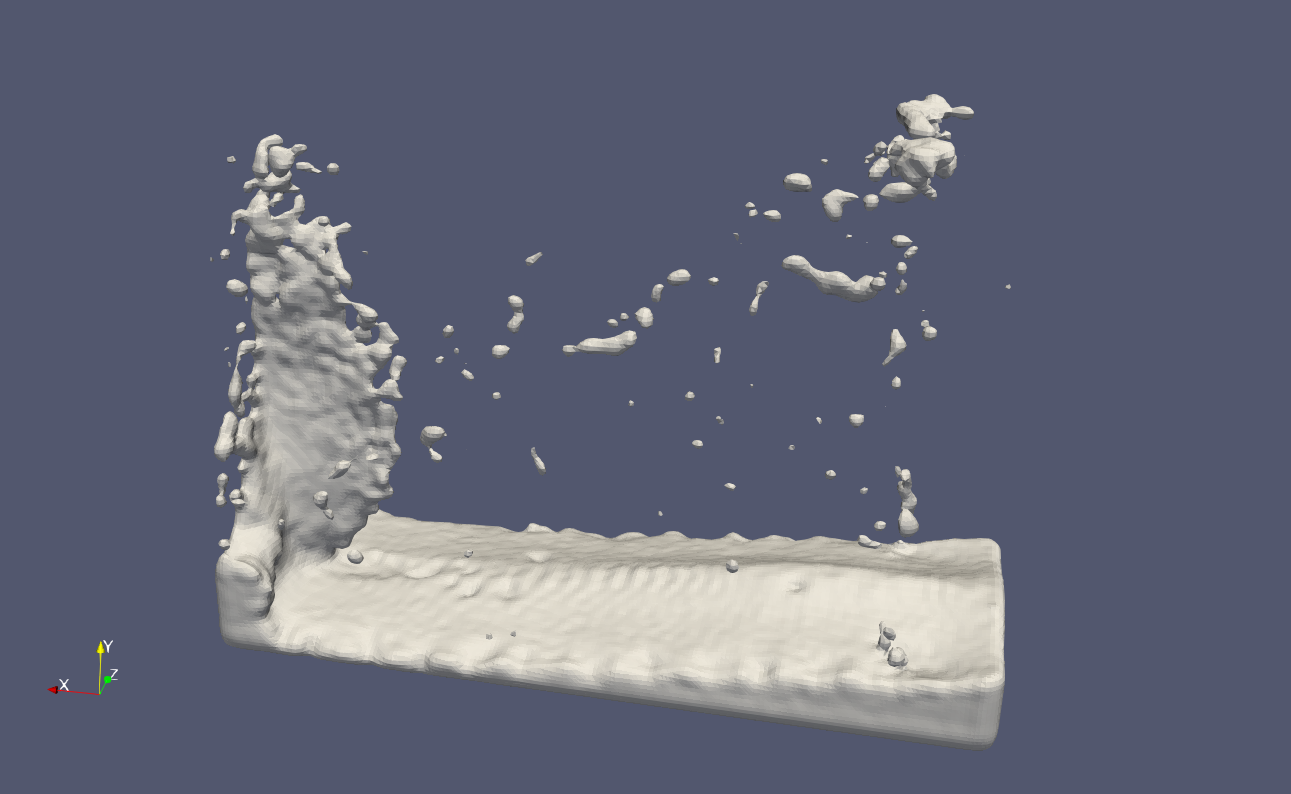
\includegraphics[width=\textwidth]{figures/ReconstructionDencityBased.png}
				\caption{Method: DB}
        \end{subfigure}
        \begin{subfigure}[b]{0.4\textwidth}
               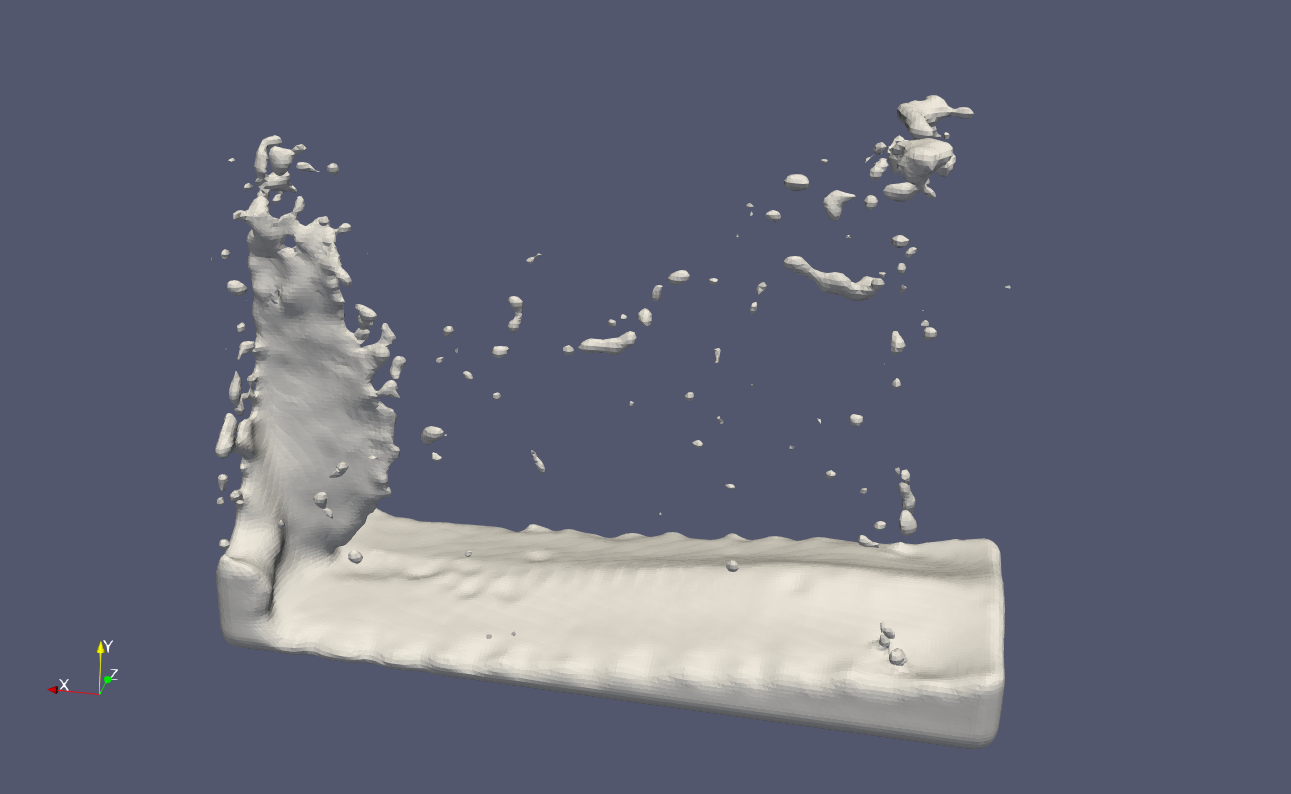
\includegraphics[width=\textwidth]{figures/ReconstructionDencityBasedBlur.png}
				\caption{Method: DBblur}
        \end{subfigure}
        \begin{subfigure}[b]{0.4\textwidth}
               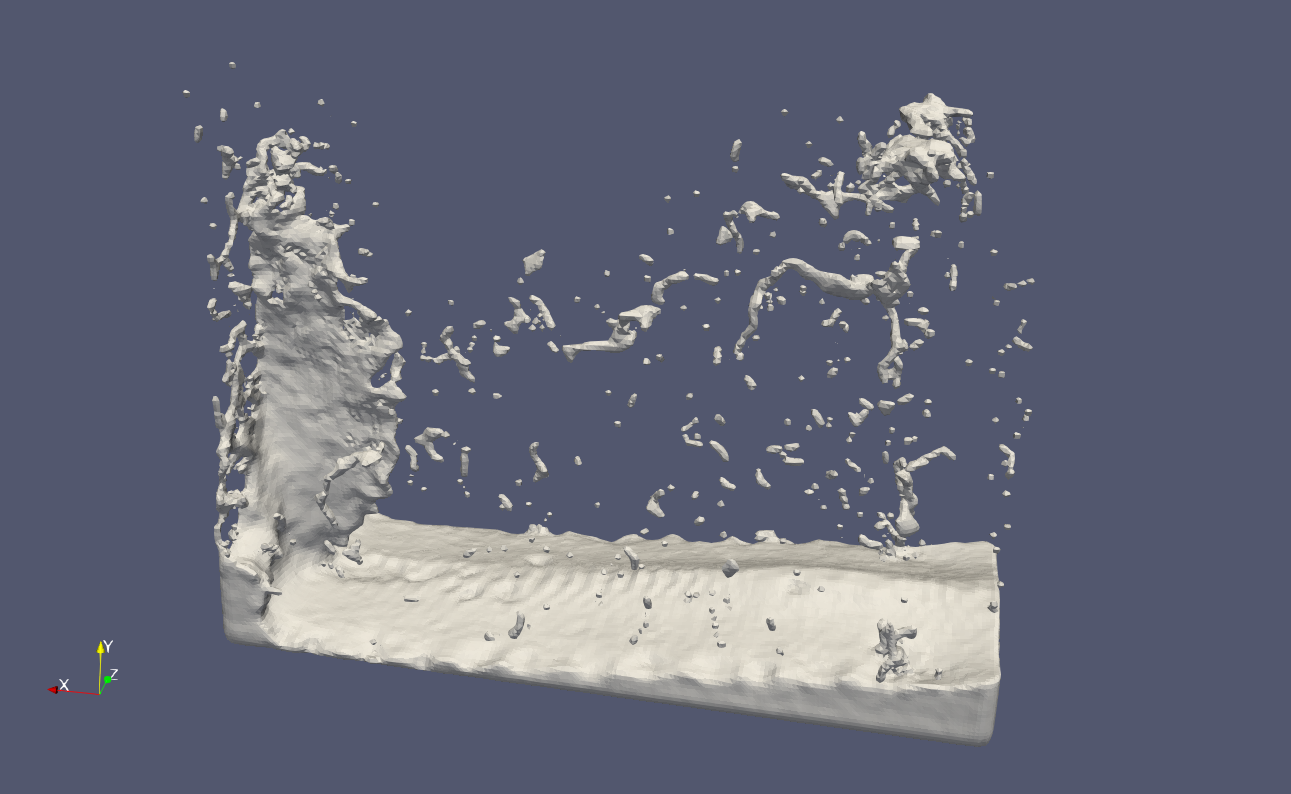
\includegraphics[width=\textwidth]{figures/ReconstructionZhuBridson.png}
				\caption{Method: ZB}
        \end{subfigure}
        \begin{subfigure}[b]{0.4\textwidth}
               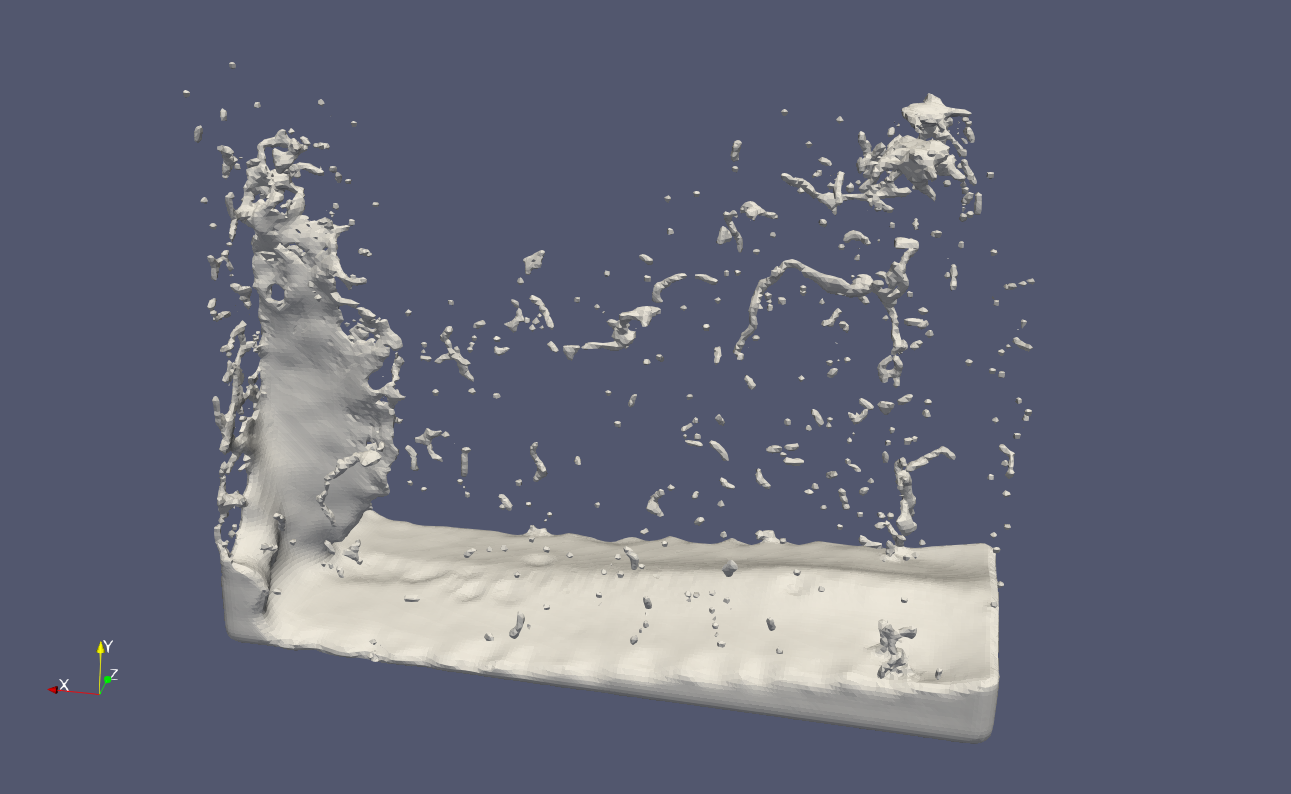
\includegraphics[width=\textwidth]{figures/ReconstructionZhuBridsonBlur.png}
				\caption{Method: ZBblur}
        \end{subfigure}
        \caption{Fluid surface comparison in dam break scene}
        \label{fig:DamBreak}
	\end{center}
\end{figure}


Another scene comparison is shown in the figure \ref{fig:MotorScene}. Particle count - 5000, particle radius - 0.025
\begin{figure}[h]
	\begin{center}
        \begin{subfigure}[b]{0.4\textwidth}
               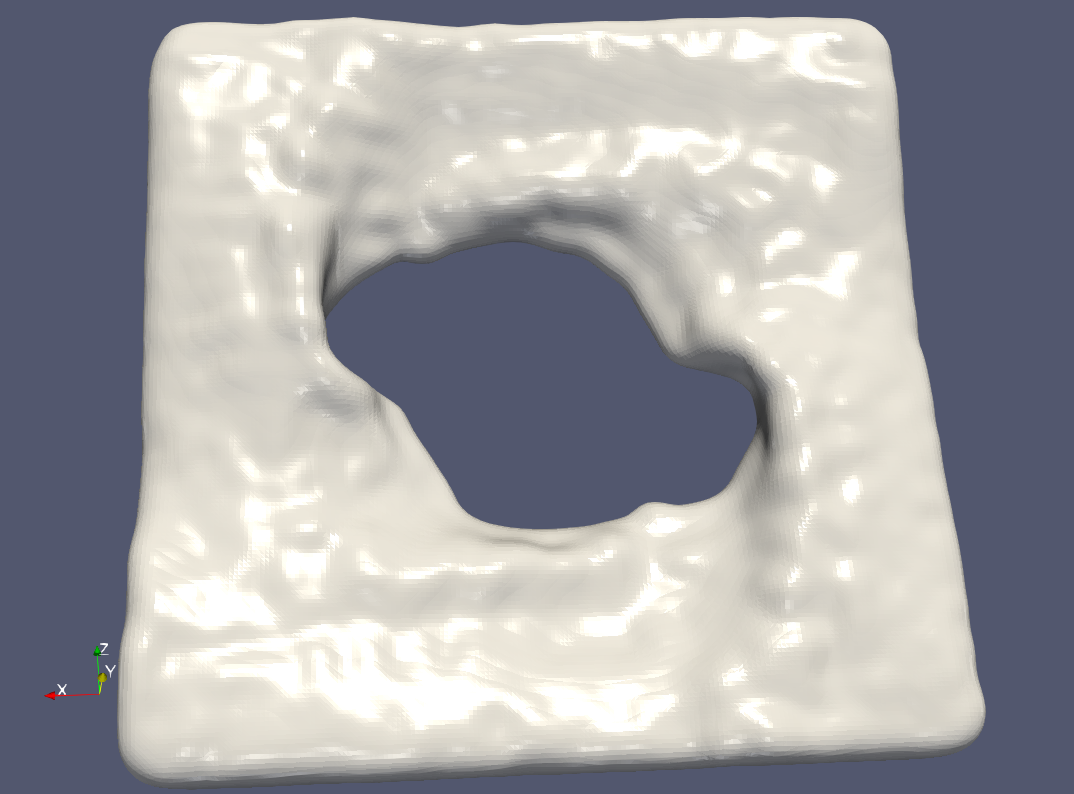
\includegraphics[width=\textwidth]{figures/ReconstructionMotorSceneDencityBased.png}
				\caption{Method: DB}
        \end{subfigure}
        \begin{subfigure}[b]{0.4\textwidth}
               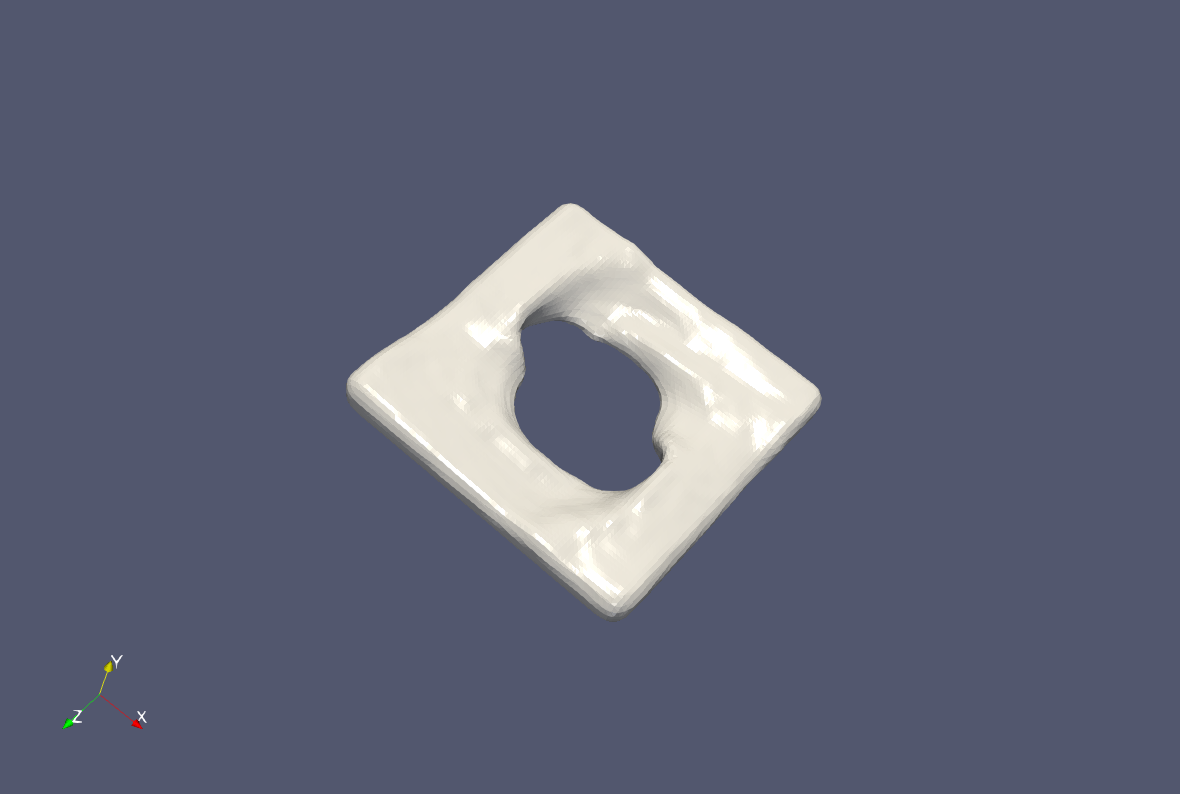
\includegraphics[width=\textwidth]{figures/ReconstructionMotorSceneDencityBasedBlur.png}
				\caption{Method: DBblur}
        \end{subfigure}
        \begin{subfigure}[b]{0.4\textwidth}
               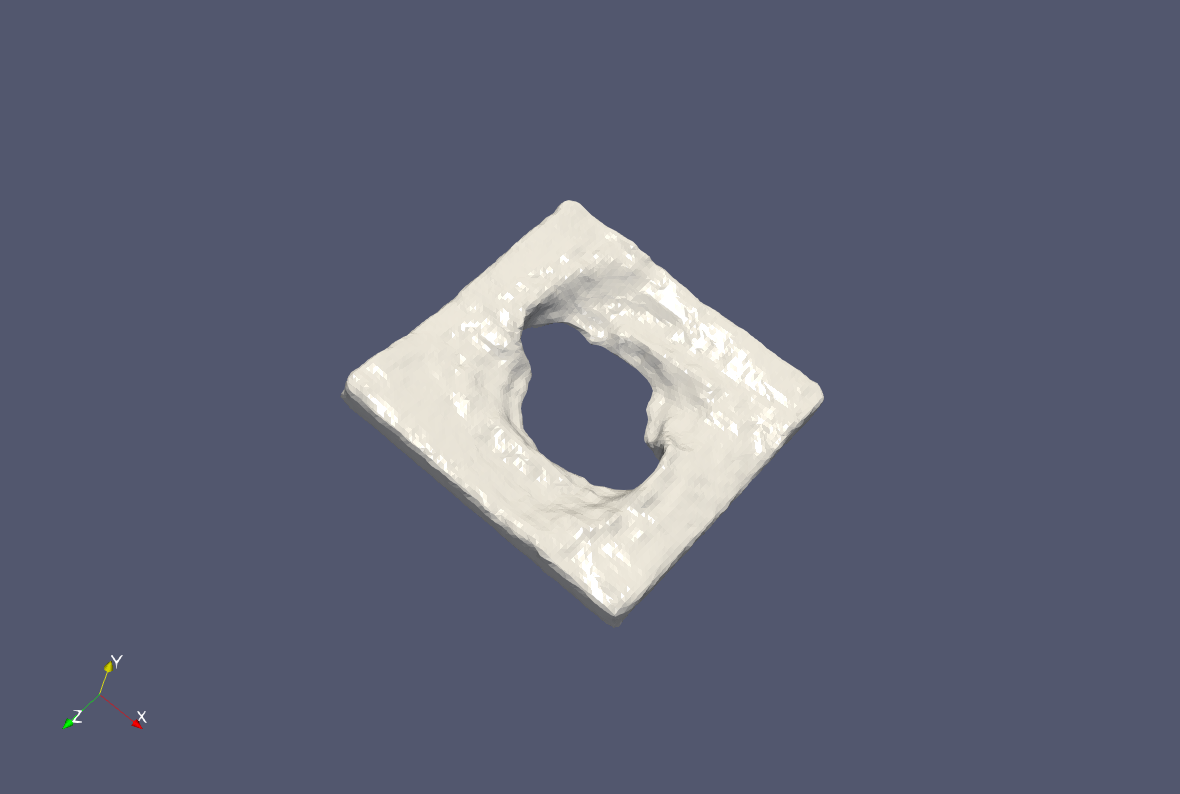
\includegraphics[width=\textwidth]{figures/ReconstructionMotorSceneZhuBridson.png}
				\caption{Method: ZB}
        \end{subfigure}
        \begin{subfigure}[b]{0.4\textwidth}
               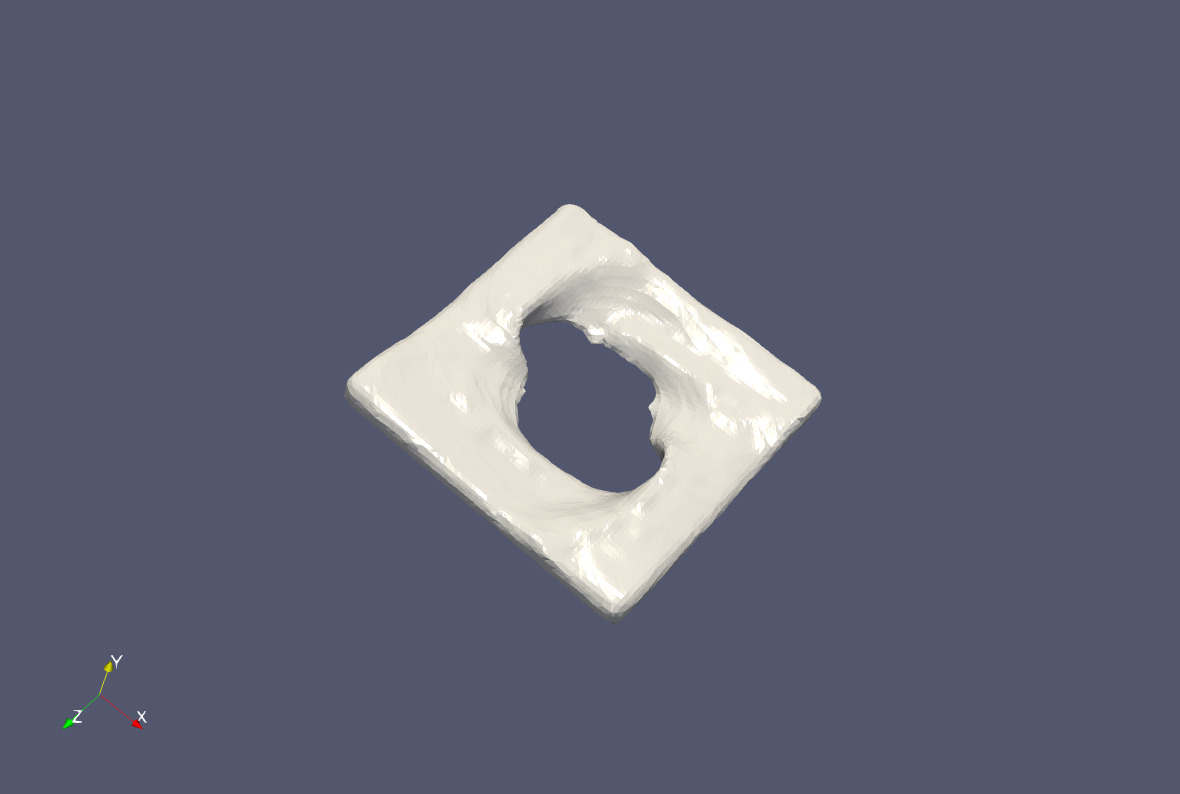
\includegraphics[width=\textwidth]{figures/ReconstructionMotorSceneZhuBridsonBlur.png}
				\caption{Method: ZBblur}
        \end{subfigure}
        \caption{Motor scene fluid surface reconstruction comparison}
        \label{fig:MotorScene}
	\end{center}
\end{figure}



\section{Conclusions}
After all experimentations performed with the developed method the conclusion can be made, that application of blur to the level set is definitely influences the final surface quality, and this method is able to smooth flat areas of surface, in the mean time saving small features in splash areas.\\
The developed algorithm is applied on top of the original reconstruction algorithm. It can be applied to every reconstruction method, which uses scalar distance field to construct iso surfaces and reconstruct the surface itself.\\ 
Further efforts can be applied to improve algorithm performance, e.g. porting blur stage on GPU.\\
However, this method still has severe drawback - a problem of parametrization. There are multiple parameters that should be tunned, such as kernel size, kernel offset, kernel depth, smoothing factor, blur iterations. For different reconstruction methods, depending on the structure of the level set, simulation scale, performance and surface quality requirements, there is no golden middle for automatic application of the parametrization. Thus manual parameters tuning is required to achieve required reconstruction quality.\\

